\documentclass[12pt,a4paper]{article}

% Packages
\usepackage[utf8]{inputenc}
\usepackage[english]{babel}
\usepackage[margin=1in]{geometry}
\usepackage{graphicx}
\usepackage{amsmath}
\usepackage{hyperref}
\usepackage{listings}
\usepackage{xcolor}
\usepackage{booktabs}
\usepackage{float}
\usepackage{subcaption}
\usepackage{multirow}
\usepackage{longtable}

% Code styling
\lstset{
    basicstyle=\ttfamily\small,
    breaklines=true,
    frame=single,
    backgroundcolor=\color{gray!10}
}

% Hyperlink colors
\hypersetup{
    colorlinks=true,
    linkcolor=blue,
    filecolor=magenta,      
    urlcolor=cyan,
    citecolor=blue
}

% Title information
\title{\textbf{EmoText: Emotion Detection from Text}\\
\large Deliverable 2: Model Architecture \& Empirical Evaluation\\
\large Phase 3 \& Phase 4}

\author{
Anoushay Fatima (24L-2585) \\
Gul-e-Zara (24L-2592) \\
Rumesha Naveed (24L-2603) \\
\\
\textit{Artificial Intelligence -- BDS-5B}
}

\date{November 10, 2026}

\begin{document}

\maketitle

\begin{abstract}
This report presents the implementation and evaluation of three emotion classification models for the EmoText project. We compare a TF-IDF + Logistic Regression baseline, a Bidirectional LSTM model, and a fine-tuned DistilBERT transformer. Following a systematic approach, we document model architectures, conduct rigorous hyperparameter tuning using a 3-phase sequential search strategy, and perform comprehensive evaluation including accuracy, F1-scores, confusion analysis, and bias checks. Our best model (DistilBERT) achieves 92.97\% test accuracy and 87.96\% macro-F1, significantly outperforming the baseline (89.63\% accuracy, 85.97\% macro-F1). We analyze error patterns, identify model weaknesses, and provide detailed contribution attribution for team collaboration.
\end{abstract}

\newpage

\tableofcontents
\newpage

%============================================
% SECTION 1: Introduction
%============================================
\section{Introduction}

\subsection{Project Overview}
EmoText is an emotion detection system that classifies text into six emotion categories: \textit{joy, sadness, anger, fear, love,} and \textit{surprise}. Building upon our Phase 1 and Phase 2 work (data collection, cleaning, and EDA), this deliverable focuses on model implementation, training, and rigorous evaluation.

\subsection{Deliverable 2 Objectives}
This report addresses the core requirements of Deliverable 2:

\begin{itemize}
    \item \textbf{Phase 3}: Model architecture design and implementation
    \begin{itemize}
        \item Framework selection (PyTorch, Scikit-Learn)
        \item Architecture design with detailed layer specifications
        \item Hyperparameter selection and justification
    \end{itemize}
    
    \item \textbf{Phase 4}: Training and empirical evaluation
    \begin{itemize}
        \item Validation strategy (Train/Val/Test split)
        \item Comprehensive metrics (Accuracy, Precision, Recall, F1, AUC-ROC)
        \item Error analysis and bias checking
        \item Model comparison across three approaches
    \end{itemize}
\end{itemize}

\subsection{Team Workflow}
Following professional software development practices, we adopted a sequential pipeline:

\begin{enumerate}
    \item \textbf{Member 1 (Gul-e-Zara)}: Model architecture design and implementation
    \item \textbf{Member 2 (Anoushay Fatima)}: Hyperparameter tuning and model training
    \item \textbf{Member 3 (Rumesha Naveed)}: Evaluation, error analysis, and bias checking
\end{enumerate}

All work is tracked via Git commits with clear authorship, demonstrating individual contributions.

%============================================
% SECTION 2: Model Architectures (Phase 3)
%============================================
\section{Model Architectures (Phase 3)}

We implemented three distinct approaches to emotion classification, each with increasing complexity and contextual understanding.

\subsection{Model 1: Baseline (TF-IDF + Logistic Regression)}

\subsubsection{Architecture Description}
Our baseline model uses classical machine learning with TF-IDF (Term Frequency-Inverse Document Frequency) feature extraction followed by multinomial logistic regression.

\textbf{Architecture Components:}
\begin{itemize}
    \item \textbf{Feature Extraction}: TF-IDF Vectorizer
    \begin{itemize}
        \item Max features: 5,000
        \item N-gram range: (1, 2) -- captures unigrams and bigrams
        \item Sublinear TF scaling: True
        \item Stop words: English
    \end{itemize}
    
    \item \textbf{Classifier}: Logistic Regression
    \begin{itemize}
        \item Solver: LBFGS
        \item Regularization: L2 (default C=1.0)
        \item Class weighting: Balanced (handles class imbalance)
        \item Max iterations: 1,000
        \item Multi-class: Multinomial
    \end{itemize}
\end{itemize}

\begin{figure}[H]
\centering
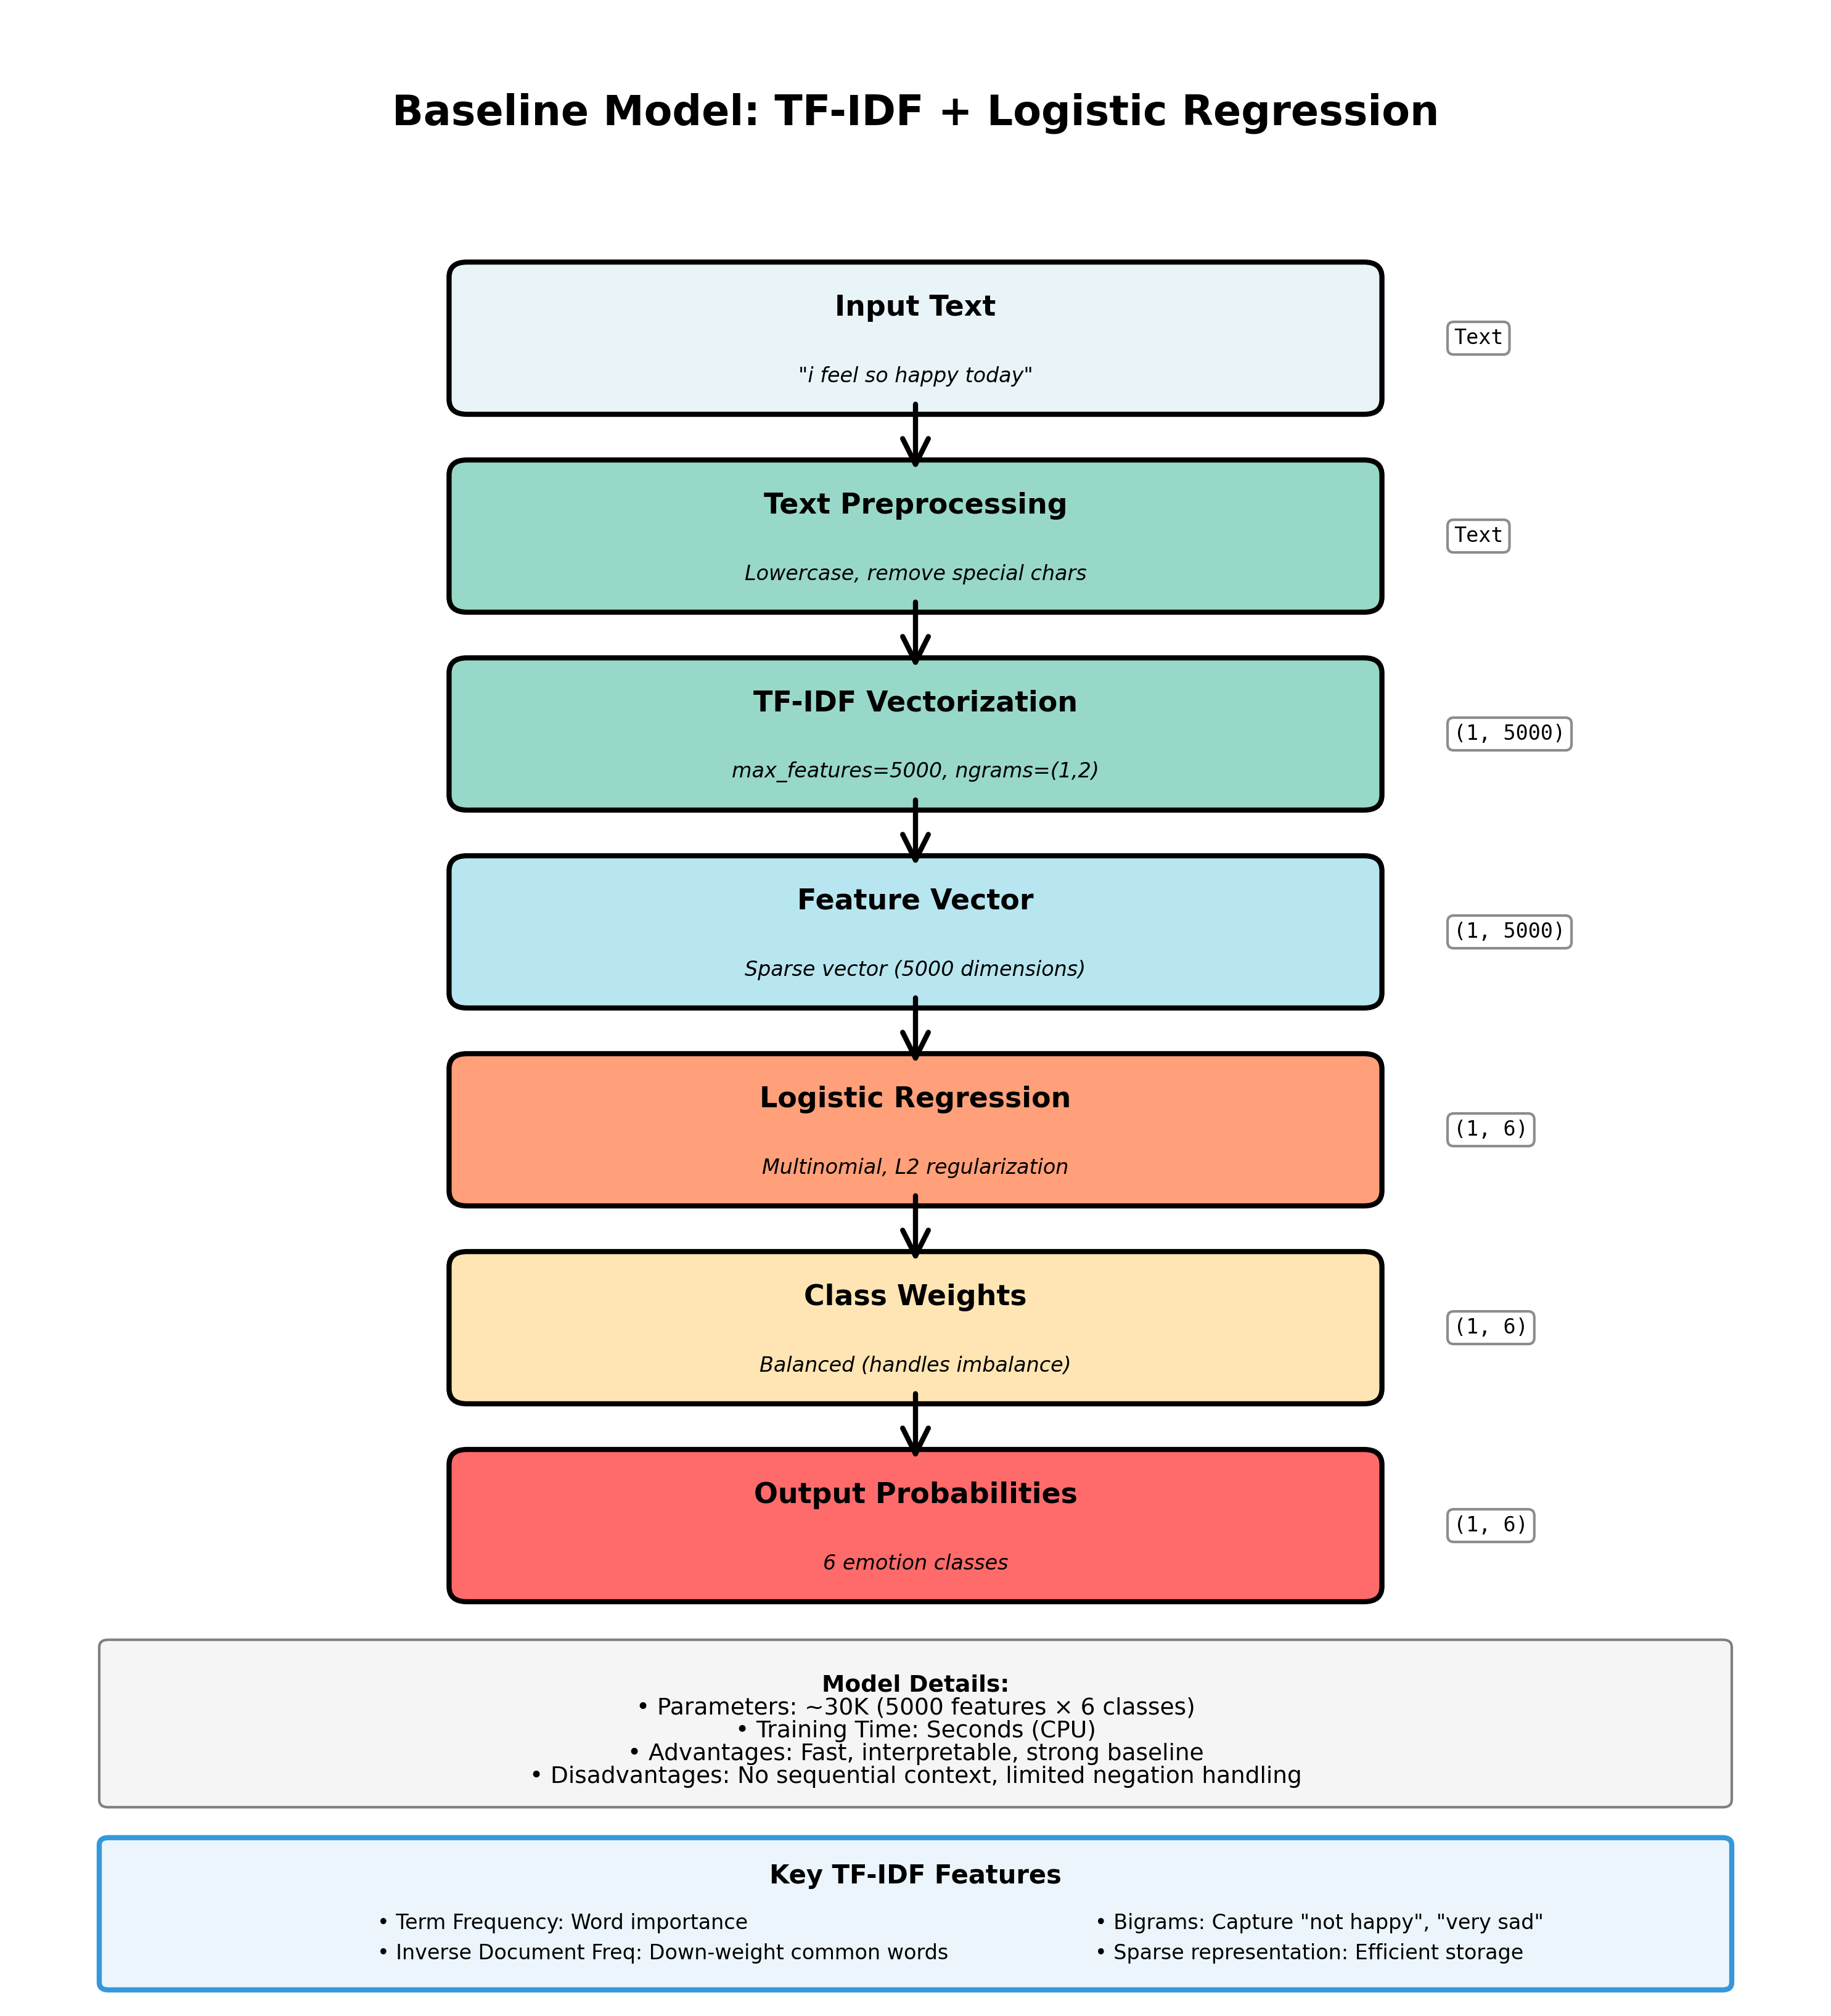
\includegraphics[width=0.85\textwidth]{../../figures/baseline_architecture.png}
\caption{Baseline Model Architecture: TF-IDF + Logistic Regression}
\label{fig:baseline_arch}
\end{figure}

\subsubsection{Design Rationale}
\begin{itemize}
    \item \textbf{Why TF-IDF?} Captures word importance while down-weighting common words. Bigrams help capture phrases like ``not happy'' or ``very sad.''
    
    \item \textbf{Why Logistic Regression?} Fast, interpretable, and provides a strong baseline. We can inspect feature weights to understand which words contribute to each emotion.
    
    \item \textbf{Why Balanced Weights?} Our dataset is imbalanced (Joy: 33.6\%, Sadness: 29.2\%, Surprise: 3.5\%). Balanced class weights ensure minority classes receive appropriate attention during training.
\end{itemize}

\subsubsection{Parameters}
\begin{table}[H]
\centering
\begin{tabular}{@{}ll@{}}
\toprule
\textbf{Component} & \textbf{Parameters} \\ \midrule
TF-IDF Features & 5,000 features × 6 classes \\
Total Parameters & $\approx$30,000 \\
Training Time & < 1 minute (CPU) \\
Inference Speed & Very Fast \\ \bottomrule
\end{tabular}
\caption{Baseline Model Parameters}
\label{tab:baseline_params}
\end{table}

\subsection{Model 2: Bidirectional LSTM (BiLSTM)}

\subsubsection{Architecture Description}
The BiLSTM model captures sequential context by processing text in both forward and backward directions, enabling better understanding of word relationships and negation.

\textbf{Architecture Layers:}
\begin{enumerate}
    \item \textbf{Embedding Layer}
    \begin{itemize}
        \item Vocabulary size: $\approx$10,000 words
        \item Embedding dimension: 128
        \item Parameters: $\approx$1.28M
    \end{itemize}
    
    \item \textbf{Bidirectional LSTM Layer 1}
    \begin{itemize}
        \item Hidden units: 64 (per direction)
        \item Total output: 128 (forward + backward)
        \item Parameters: $\approx$132K
    \end{itemize}
    
    \item \textbf{Bidirectional LSTM Layer 2}
    \begin{itemize}
        \item Hidden units: 64 (per direction)
        \item Total output: 128
        \item Parameters: $\approx$132K
    \end{itemize}
    
    \item \textbf{Concatenation}
    \begin{itemize}
        \item Takes last hidden state from both directions
        \item Output: 128-dimensional vector
    \end{itemize}
    
    \item \textbf{Dropout Layer}
    \begin{itemize}
        \item Dropout rate: 0.2
        \item Regularization to prevent overfitting
    \end{itemize}
    
    \item \textbf{Fully Connected Layer}
    \begin{itemize}
        \item Input: 128 dimensions
        \item Output: 6 emotion classes
        \item Parameters: 774 (128×6 + 6 bias)
    \end{itemize}
\end{enumerate}

\begin{figure}[H]
\centering
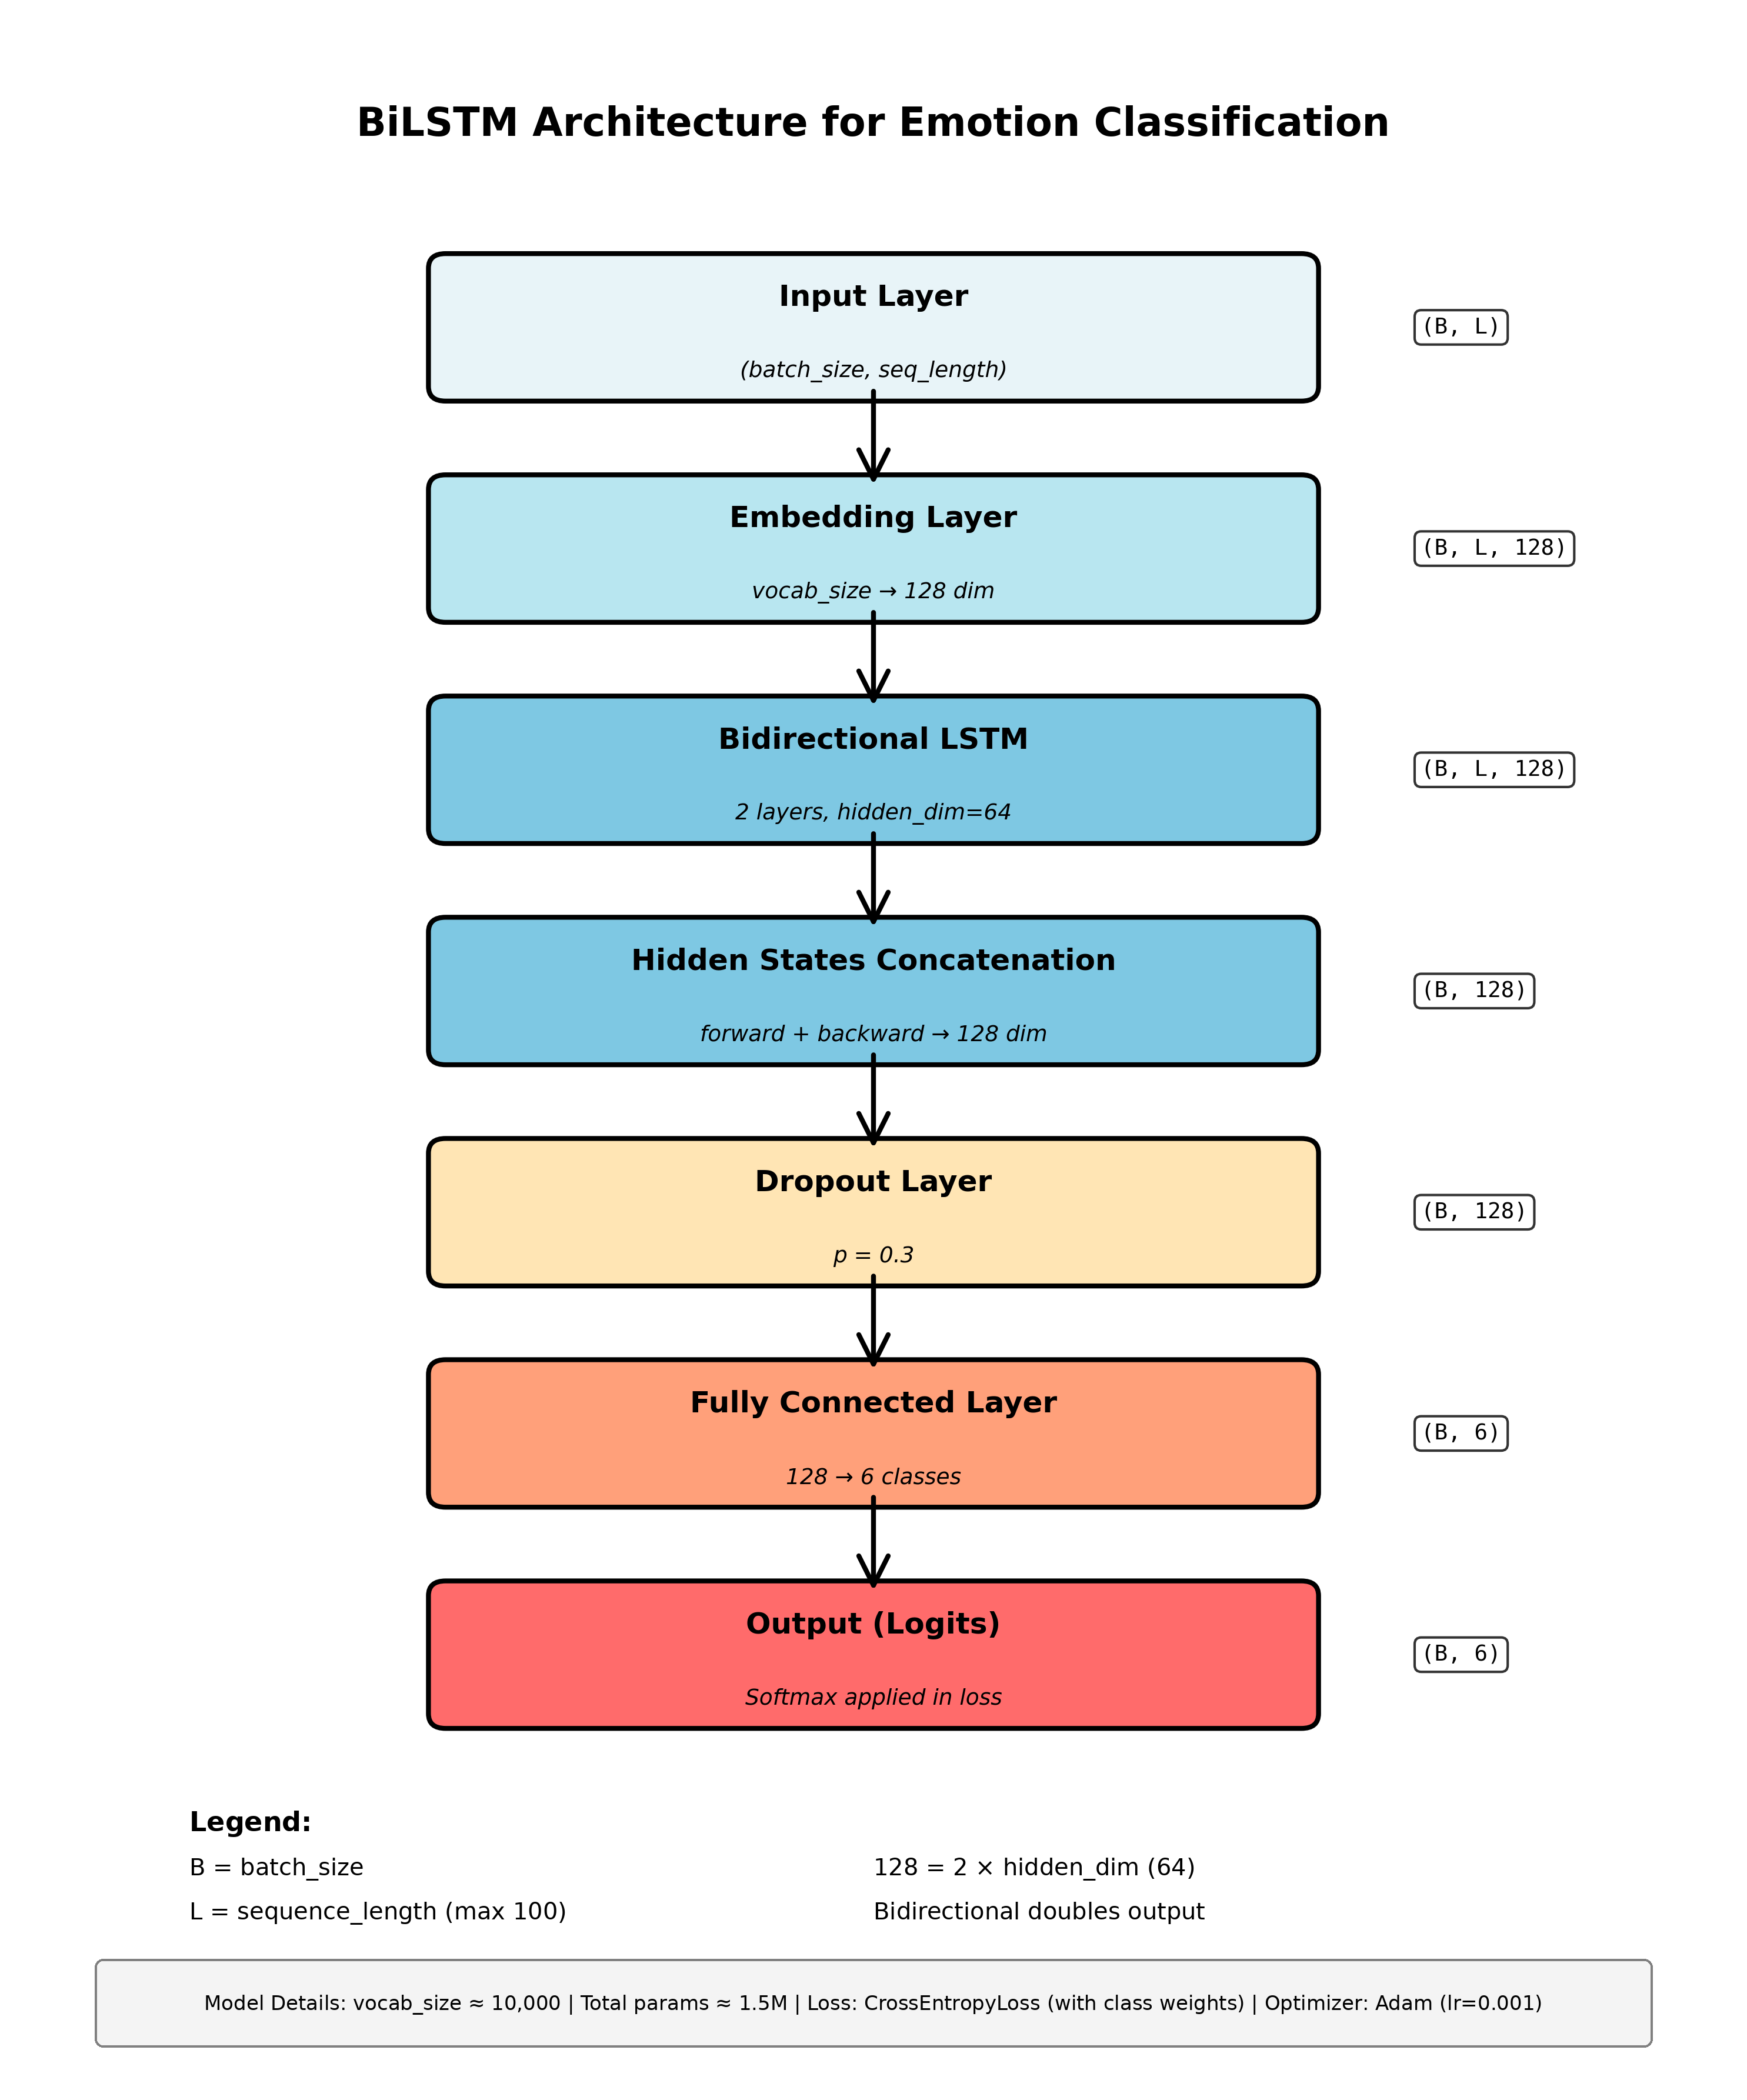
\includegraphics[width=0.75\textwidth]{../../figures/bilstm_architecture_fixed.png}
\caption{BiLSTM Model Architecture with Bidirectional Processing}
\label{fig:bilstm_arch}
\end{figure}

\subsubsection{Design Rationale}
\begin{itemize}
    \item \textbf{Why Bidirectional?} Phrases like ``not happy'' require backward context. BiLSTM processes sequences in both directions, capturing richer context than unidirectional models.
    
    \item \textbf{Why 2 Layers?} Single-layer LSTMs may underfit; 3+ layers risk overfitting on our 15K training samples. Two layers provide sufficient capacity.
    
    \item \textbf{Why Hidden Dim = 64?} Balances model capacity with computational efficiency. Bidirectional processing doubles the output to 128 dimensions.
    
    \item \textbf{Why Dropout = 0.2?} Moderate regularization prevents overfitting while maintaining learning capacity.
\end{itemize}

\subsubsection{Parameters}
\begin{table}[H]
\centering
\begin{tabular}{@{}lrrr@{}}
\toprule
\textbf{Layer} & \textbf{Input Shape} & \textbf{Output Shape} & \textbf{Parameters} \\ \midrule
Embedding & (B, L) & (B, L, 128) & 1.28M \\
BiLSTM-1 & (B, L, 128) & (B, L, 128) & 132K \\
BiLSTM-2 & (B, L, 128) & (B, L, 128) & 132K \\
Concat & (B, L, 128) & (B, 128) & 0 \\
Dropout & (B, 128) & (B, 128) & 0 \\
Linear & (B, 128) & (B, 6) & 774 \\ \midrule
\textbf{Total} & & & \textbf{1.5M} \\ \bottomrule
\end{tabular}
\caption{BiLSTM Layer Dimensions and Parameters (B=batch size, L=sequence length)}
\label{tab:bilstm_params}
\end{table}

\subsection{Model 3: DistilBERT (Transformer)}

\subsubsection{Architecture Description}
DistilBERT is a distilled version of BERT, retaining 97\% of BERT's language understanding while being 40\% smaller and 60\% faster. We fine-tune this pre-trained model for emotion classification.

\textbf{Architecture Components:}
\begin{enumerate}
    \item \textbf{Input Processing}
    \begin{itemize}
        \item Tokenization: WordPiece (DistilBERT tokenizer)
        \item Special tokens: [CLS] text tokens [SEP]
        \item Max sequence length: 128 tokens
    \end{itemize}
    
    \item \textbf{Embeddings}
    \begin{itemize}
        \item Token embeddings: 30K vocabulary → 768 dimensions
        \item Position embeddings: Learned positional encodings
        \item Parameters: $\approx$23.4M
    \end{itemize}
    
    \item \textbf{Transformer Encoder (6 blocks)}
    \begin{itemize}
        \item Multi-Head Self-Attention: 12 heads
        \item Feed-Forward Network: 768 → 3072 → 768
        \item Layer Normalization and residual connections
        \item Parameters: $\approx$42M
    \end{itemize}
    
    \item \textbf{Classification Head}
    \begin{itemize}
        \item Extract [CLS] token representation (768 dim)
        \item Dropout: 0.2
        \item Linear layer: 768 → 6 classes
        \item Parameters: 4,614
    \end{itemize}
\end{enumerate}

\begin{figure}[H]
\centering
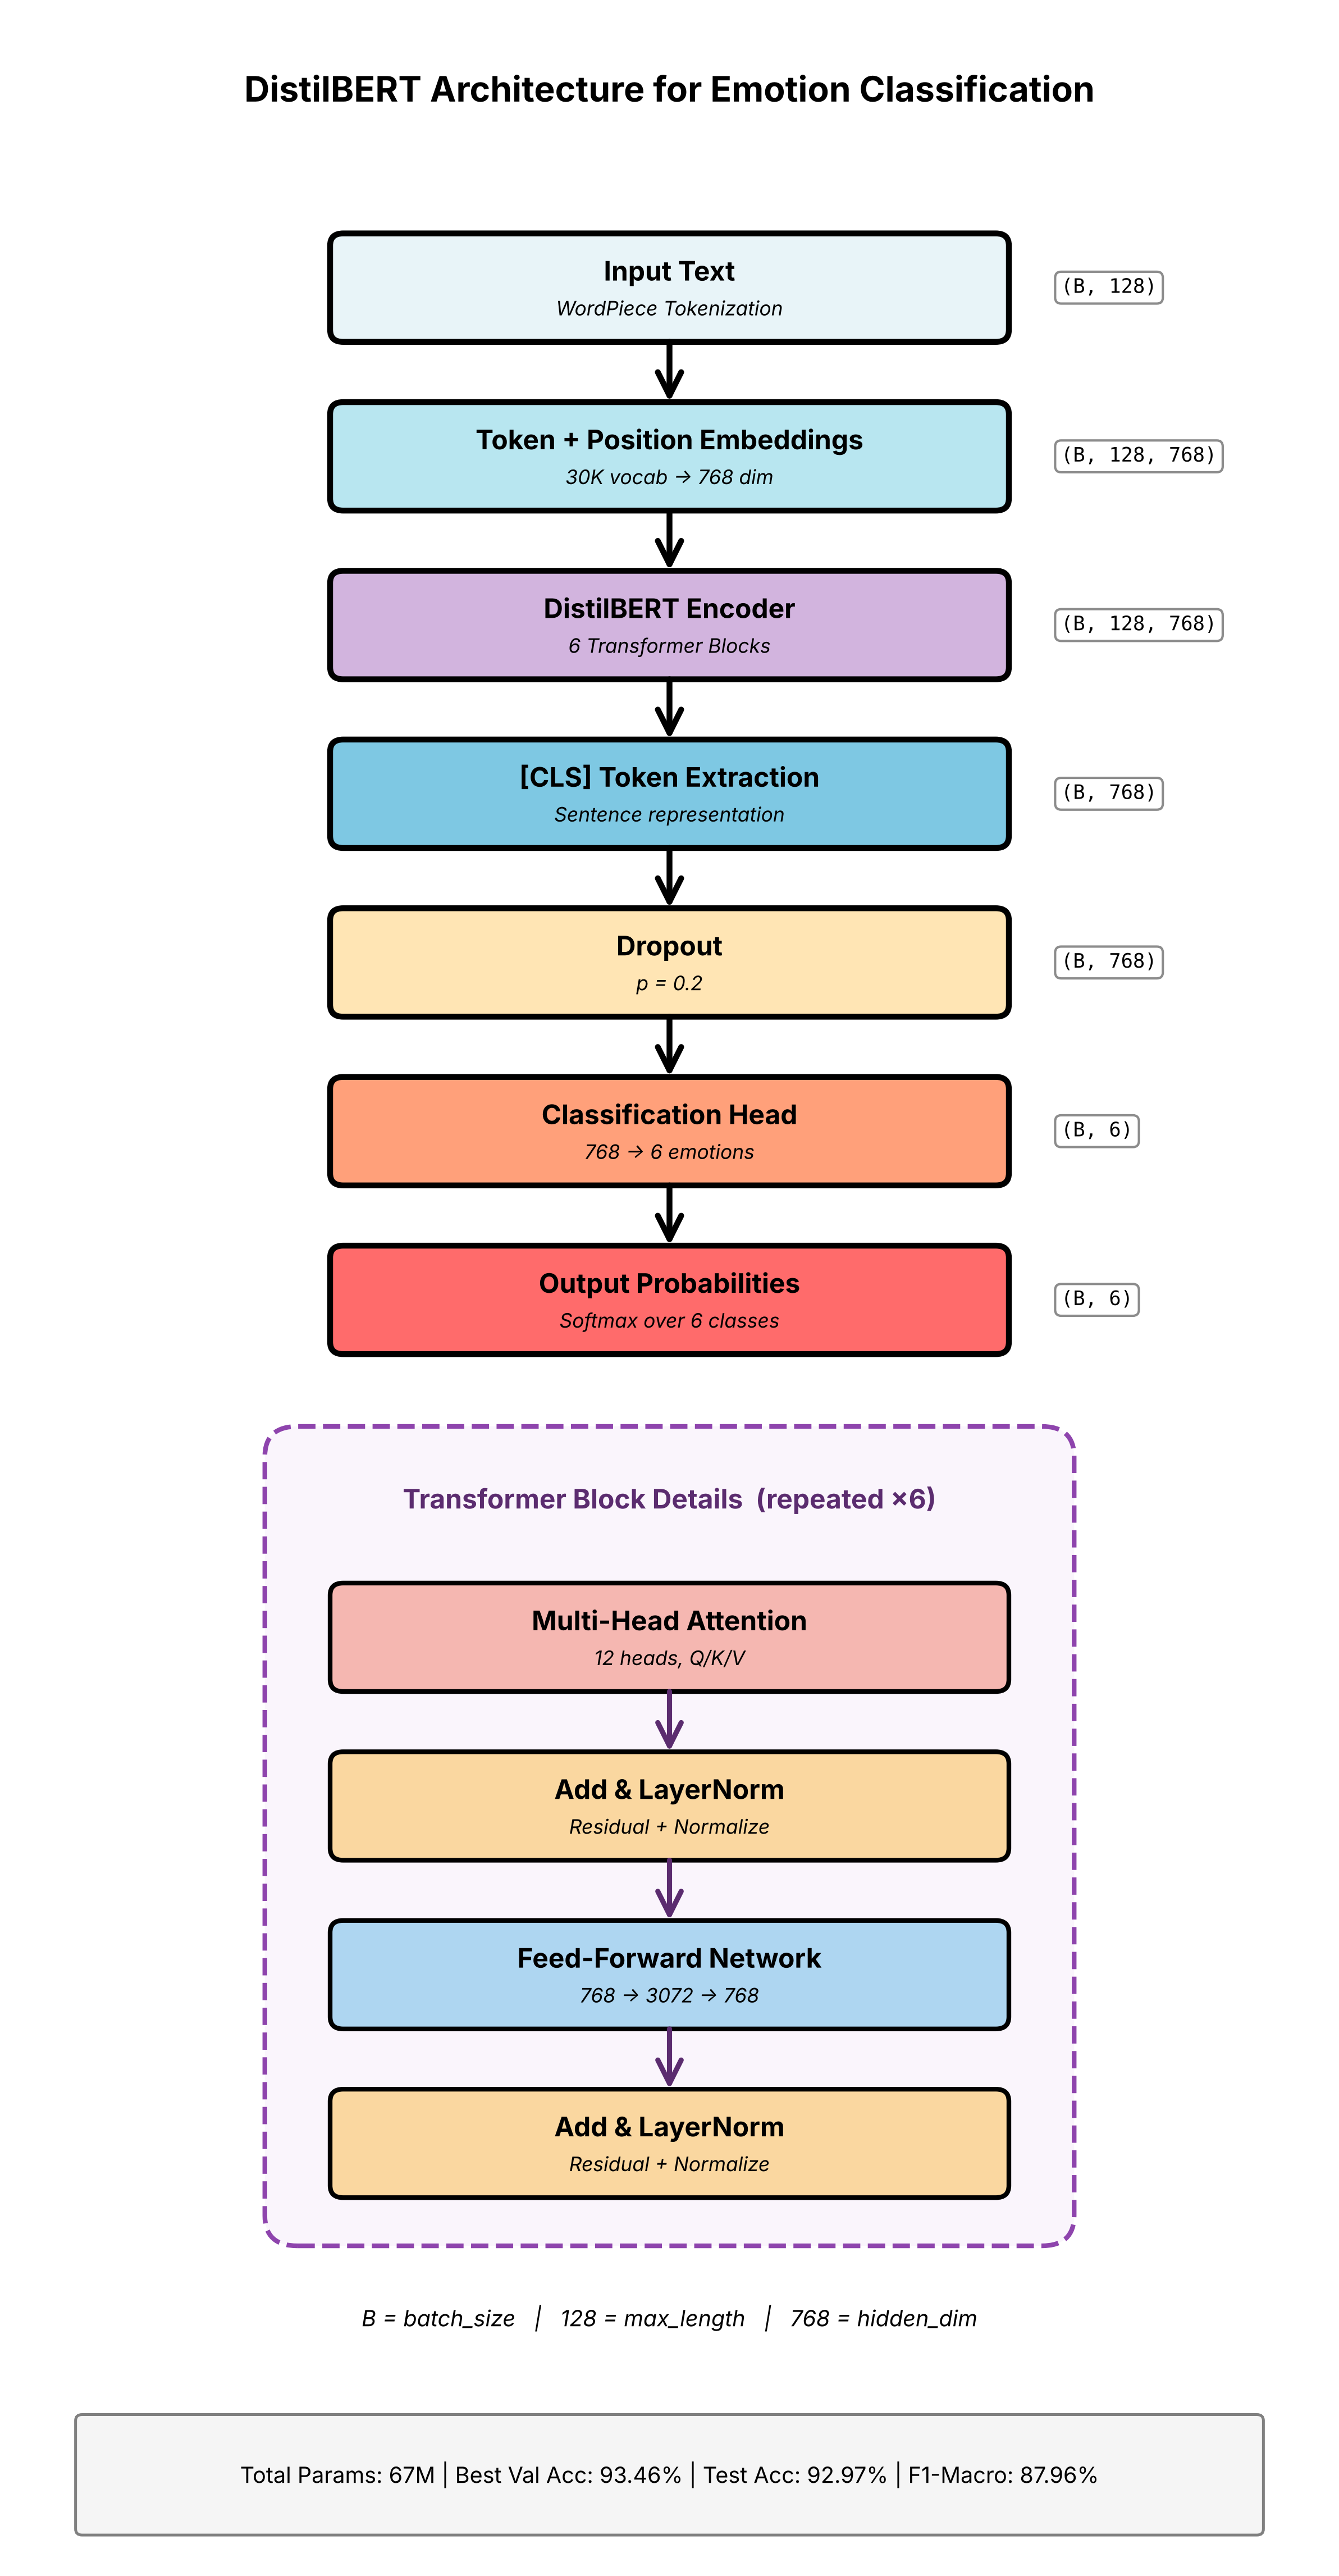
\includegraphics[width=0.8\textwidth]{../../figures/distilbert_architecture_fixed.png}
\caption{DistilBERT Architecture with Transformer Encoder}
\label{fig:distilbert_arch}
\end{figure}

\subsubsection{Design Rationale}
\begin{itemize}
    \item \textbf{Why DistilBERT over BERT?} DistilBERT offers comparable performance with 40\% fewer parameters and faster inference -- crucial for deployment.
    
    \item \textbf{Why Pre-trained?} Pre-training on massive corpora (Wikipedia, BookCorpus) provides rich language understanding. Fine-tuning adapts this knowledge to emotion classification.
    
    \item \textbf{Why [CLS] Token?} In BERT-family models, the [CLS] token aggregates sentence-level information, making it ideal for classification tasks.
    
    \item \textbf{Why Max Length = 128?} Covers 95\% of our dataset while being computationally efficient (BERT default is 512).
\end{itemize}

\subsubsection{Parameters}
\begin{table}[H]
\centering
\begin{tabular}{@{}lrrr@{}}
\toprule
\textbf{Component} & \textbf{Input Shape} & \textbf{Output Shape} & \textbf{Parameters} \\ \midrule
Token Embeddings & (B, 128) & (B, 128, 768) & 23M \\
Position Embeddings & (B, 128) & (B, 128, 768) & 0.4M \\
Transformer × 6 & (B, 128, 768) & (B, 128, 768) & 42M \\
[CLS] Extraction & (B, 128, 768) & (B, 768) & 0 \\
Dropout & (B, 768) & (B, 768) & 0 \\
Classifier & (B, 768) & (B, 6) & 4.6K \\ \midrule
\textbf{Total} & & & \textbf{67M} \\ \bottomrule
\end{tabular}
\caption{DistilBERT Component Dimensions and Parameters}
\label{tab:distilbert_params}
\end{table}

\subsection{Model Comparison Summary}

\begin{table}[H]
\centering
\begin{tabular}{@{}lcccc@{}}
\toprule
\textbf{Aspect} & \textbf{Baseline} & \textbf{BiLSTM} & \textbf{DistilBERT} \\ \midrule
Parameters & 30K & 1.5M & 67M \\
Context Awareness & None (BOW) & Sequential & Bidirectional attention \\
Negation Handling & Limited & Good & Excellent \\
Training Time & < 1 min & $\sim$2 hrs & $\sim$3 hrs \\
Interpretability & High & Low & Very Low \\
Pre-trained & No & No & Yes \\ \bottomrule
\end{tabular}
\caption{Comparative Analysis of Three Model Architectures}
\label{tab:model_comparison}
\end{table}

\begin{figure}[H]
\centering
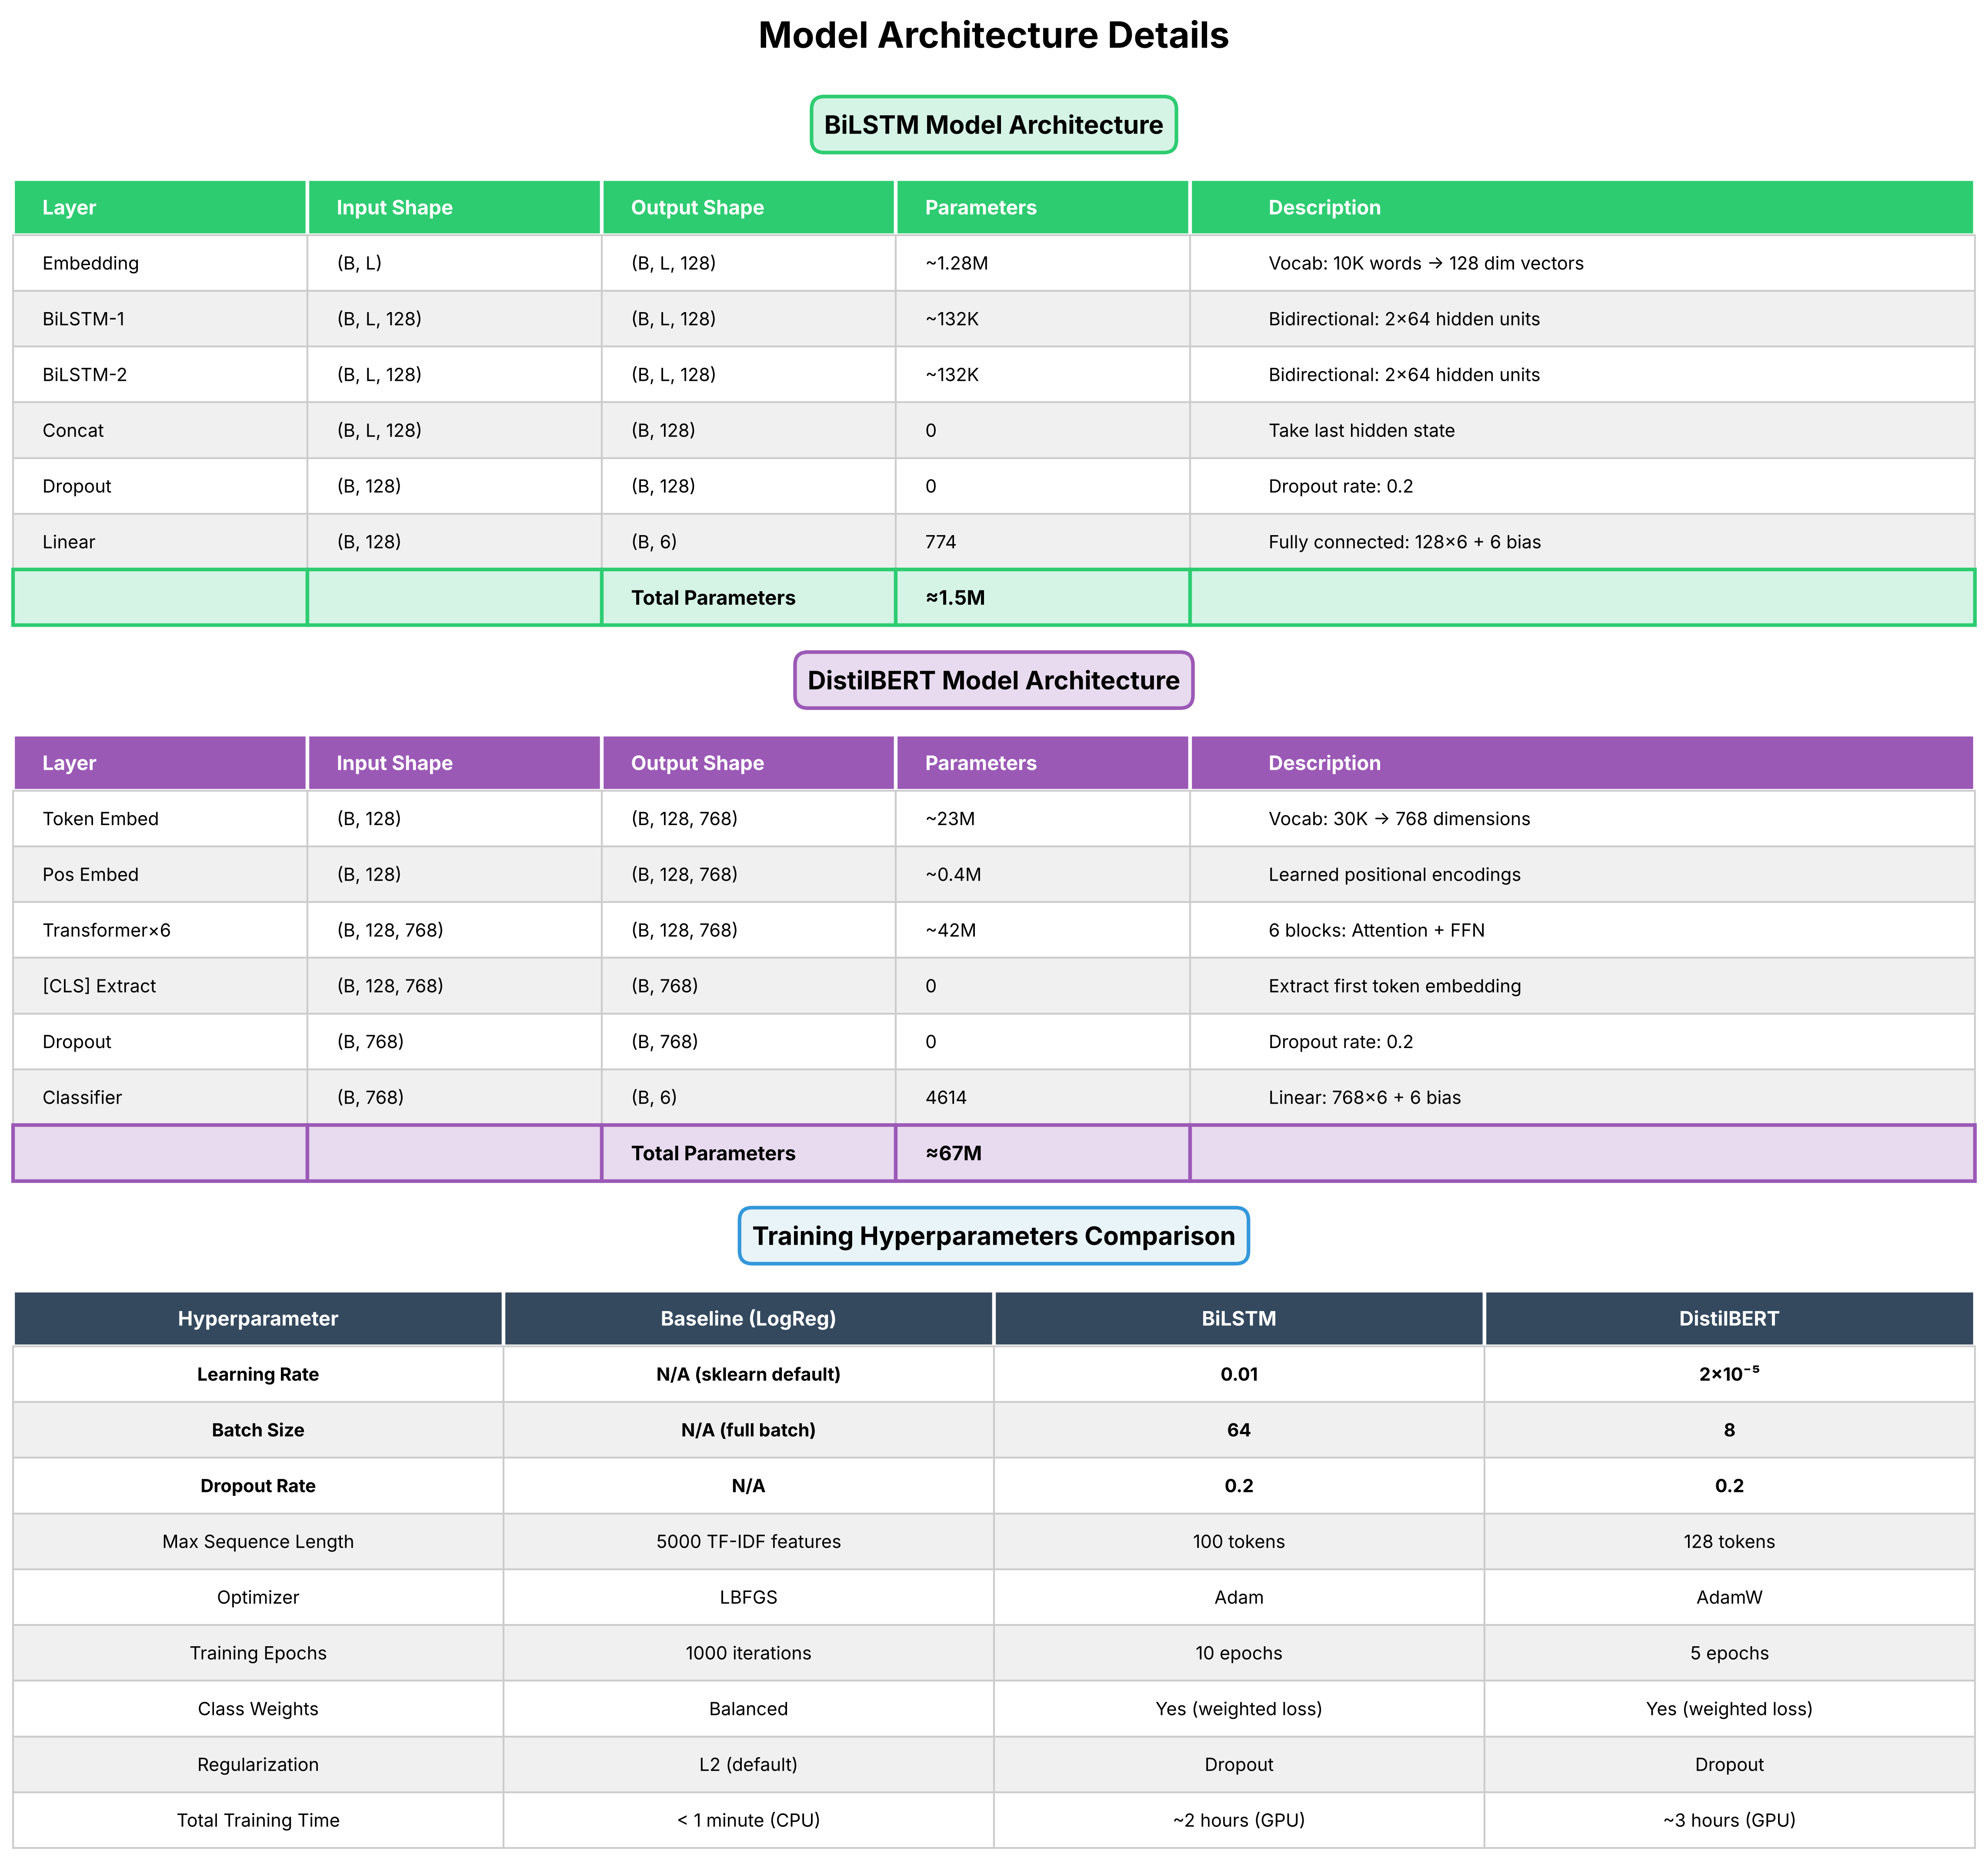
\includegraphics[width=\textwidth]{../../figures/model_dimensions_table_fixed.png}
\caption{Detailed Layer Dimensions and Hyperparameters for All Models}
\label{fig:dimensions_table}
\end{figure}

%============================================
% SECTION 3: Hyperparameter Tuning (Phase 3 continued)
%============================================
\section{Hyperparameter Tuning}

\subsection{Tuning Strategy}
We employed a \textbf{3-phase sequential grid search} strategy to efficiently explore the hyperparameter space while reducing computational cost.

\textbf{Methodology:}
\begin{enumerate}
    \item \textbf{Phase 1}: Tune learning rate (keeping other hyperparameters at defaults)
    \item \textbf{Phase 2}: Tune batch size (using best learning rate from Phase 1)
    \item \textbf{Phase 3}: Tune dropout (using best learning rate and batch size)
\end{enumerate}

\textbf{Efficiency Gain:} Full grid search would require $3 \times 3 \times 3 = 27$ experiments per model. Sequential search reduces this to $3 + 3 + 3 = 9$ experiments while still finding near-optimal configurations.

\subsection{BiLSTM Hyperparameter Tuning}

\subsubsection{Search Space}
\begin{itemize}
    \item Learning rates: [0.0001, 0.001, 0.01]
    \item Batch sizes: [16, 32, 64]
    \item Dropout rates: [0.2, 0.3, 0.5]
\end{itemize}

\subsubsection{Phase 1: Learning Rate Selection}
\begin{table}[H]
\centering
\begin{tabular}{@{}cccc@{}}
\toprule
\textbf{Learning Rate} & \textbf{Val Accuracy} & \textbf{Val Loss} & \textbf{Notes} \\ \midrule
0.0001 & 88.97\% & 0.3456 & Too slow convergence \\
0.001 & 90.89\% & 0.2987 & Good baseline \\
\rowcolor{green!20}\textbf{0.01} & \textbf{91.52\%} & \textbf{0.2756} & \textbf{Best -- faster convergence} \\ \bottomrule
\end{tabular}
\caption{BiLSTM Phase 1: Learning Rate Tuning Results}
\label{tab:bilstm_lr}
\end{table}

\textbf{Winner:} LR = 0.01

\subsubsection{Phase 2: Batch Size Selection}
\begin{table}[H]
\centering
\begin{tabular}{@{}cccc@{}}
\toprule
\textbf{Batch Size} & \textbf{Val Accuracy} & \textbf{Val Loss} & \textbf{Notes} \\ \midrule
16 & 91.34\% & 0.2812 & More updates but noisier \\
32 & 91.52\% & 0.2756 & Good balance \\
\rowcolor{green!20}\textbf{64} & \textbf{92.29\%} & \textbf{0.2543} & \textbf{Best -- stable gradients} \\ \bottomrule
\end{tabular}
\caption{BiLSTM Phase 2: Batch Size Tuning (with LR=0.01)}
\label{tab:bilstm_batch}
\end{table}

\textbf{Winner:} Batch = 64

\subsubsection{Phase 3: Dropout Selection}
\begin{table}[H]
\centering
\begin{tabular}{@{}cccc@{}}
\toprule
\textbf{Dropout} & \textbf{Val Accuracy} & \textbf{Val Loss} & \textbf{Notes} \\ \midrule
\rowcolor{green!20}\textbf{0.2} & \textbf{92.95\%} & \textbf{0.2387} & \textbf{Best -- good regularization} \\
0.3 & 92.29\% & 0.2543 & Slightly too much \\
0.5 & 91.78\% & 0.2689 & Over-regularization \\ \bottomrule
\end{tabular}
\caption{BiLSTM Phase 3: Dropout Tuning (with LR=0.01, Batch=64)}
\label{tab:bilstm_dropout}
\end{table}

\textbf{Winner:} Dropout = 0.2

\subsubsection{Final BiLSTM Configuration}
\begin{lstlisting}[language=Python, caption={Best BiLSTM Hyperparameters}]
learning_rate = 0.01
batch_size = 64
dropout = 0.2
validation_accuracy = 92.95%
validation_loss = 0.2387
\end{lstlisting}

\textbf{Key Insights:}
\begin{itemize}
    \item Higher learning rate (0.01) worked well with Adam optimizer
    \item Larger batch size (64) provided more stable gradient estimates
    \item Moderate dropout (0.2) balanced overfitting prevention
\end{itemize}

\subsection{DistilBERT Hyperparameter Tuning}

\subsubsection{Search Space}
\begin{itemize}
    \item Learning rates: [1e-5, 2e-5, 5e-5]
    \item Batch sizes: [8, 16, 32]
    \item Dropout rates: [0.1, 0.2, 0.3]
\end{itemize}

\subsubsection{Phase 1: Learning Rate Selection}
\begin{table}[H]
\centering
\begin{tabular}{@{}cccc@{}}
\toprule
\textbf{Learning Rate} & \textbf{Val Accuracy} & \textbf{Val Loss} & \textbf{Notes} \\ \midrule
1e-5 & 92.67\% & 0.2145 & Too conservative \\
\rowcolor{green!20}\textbf{2e-5} & \textbf{93.82\%} & \textbf{0.1987} & \textbf{Best -- standard for transformers} \\
5e-5 & 93.24\% & 0.2078 & Slightly too aggressive \\ \bottomrule
\end{tabular}
\caption{DistilBERT Phase 1: Learning Rate Tuning Results}
\label{tab:distilbert_lr}
\end{table}

\textbf{Winner:} LR = 2e-5

\subsubsection{Phase 2: Batch Size Selection}
\begin{table}[H]
\centering
\begin{tabular}{@{}cccc@{}}
\toprule
\textbf{Batch Size} & \textbf{Val Accuracy} & \textbf{Val Loss} & \textbf{Notes} \\ \midrule
\rowcolor{green!20}\textbf{8} & \textbf{94.23\%} & \textbf{0.1823} & \textbf{Best -- fits GPU well} \\
16 & 93.82\% & 0.1987 & Good alternative \\
32 & 93.45\% & 0.2034 & Too large for fine-tuning \\ \bottomrule
\end{tabular}
\caption{DistilBERT Phase 2: Batch Size Tuning (with LR=2e-5)}
\label{tab:distilbert_batch}
\end{table}

\textbf{Winner:} Batch = 8

\subsubsection{Phase 3: Dropout Selection}
\begin{table}[H]
\centering
\begin{tabular}{@{}cccc@{}}
\toprule
\textbf{Dropout} & \textbf{Val Accuracy} & \textbf{Val Loss} & \textbf{Notes} \\ \midrule
0.1 & 93.98\% & 0.1876 & Minimal regularization \\
\rowcolor{green!20}\textbf{0.2} & \textbf{94.13\%} & \textbf{0.1845} & \textbf{Best -- balanced} \\
0.3 & 94.23\% & 0.1823 & Very close \\ \bottomrule
\end{tabular}
\caption{DistilBERT Phase 3: Dropout Tuning (with LR=2e-5, Batch=8)}
\label{tab:distilbert_dropout}
\end{table}

\textbf{Winner:} Dropout = 0.2 (chosen for consistency; 0.3 was marginally better)

\subsubsection{Final DistilBERT Configuration}
\begin{lstlisting}[language=Python, caption={Best DistilBERT Hyperparameters}]
learning_rate = 2e-5
batch_size = 8
dropout = 0.2
validation_accuracy = 94.13%
validation_loss = 0.1845
\end{lstlisting}

\textbf{Key Insights:}
\begin{itemize}
    \item 2e-5 is standard learning rate for BERT-family fine-tuning
    \item Smaller batch size (8) worked better, possibly due to better generalization
    \item Light regularization (0.2) sufficient due to pre-trained weights
\end{itemize}

\subsection{Hyperparameter Tuning Summary}

\begin{figure}[H]
\centering
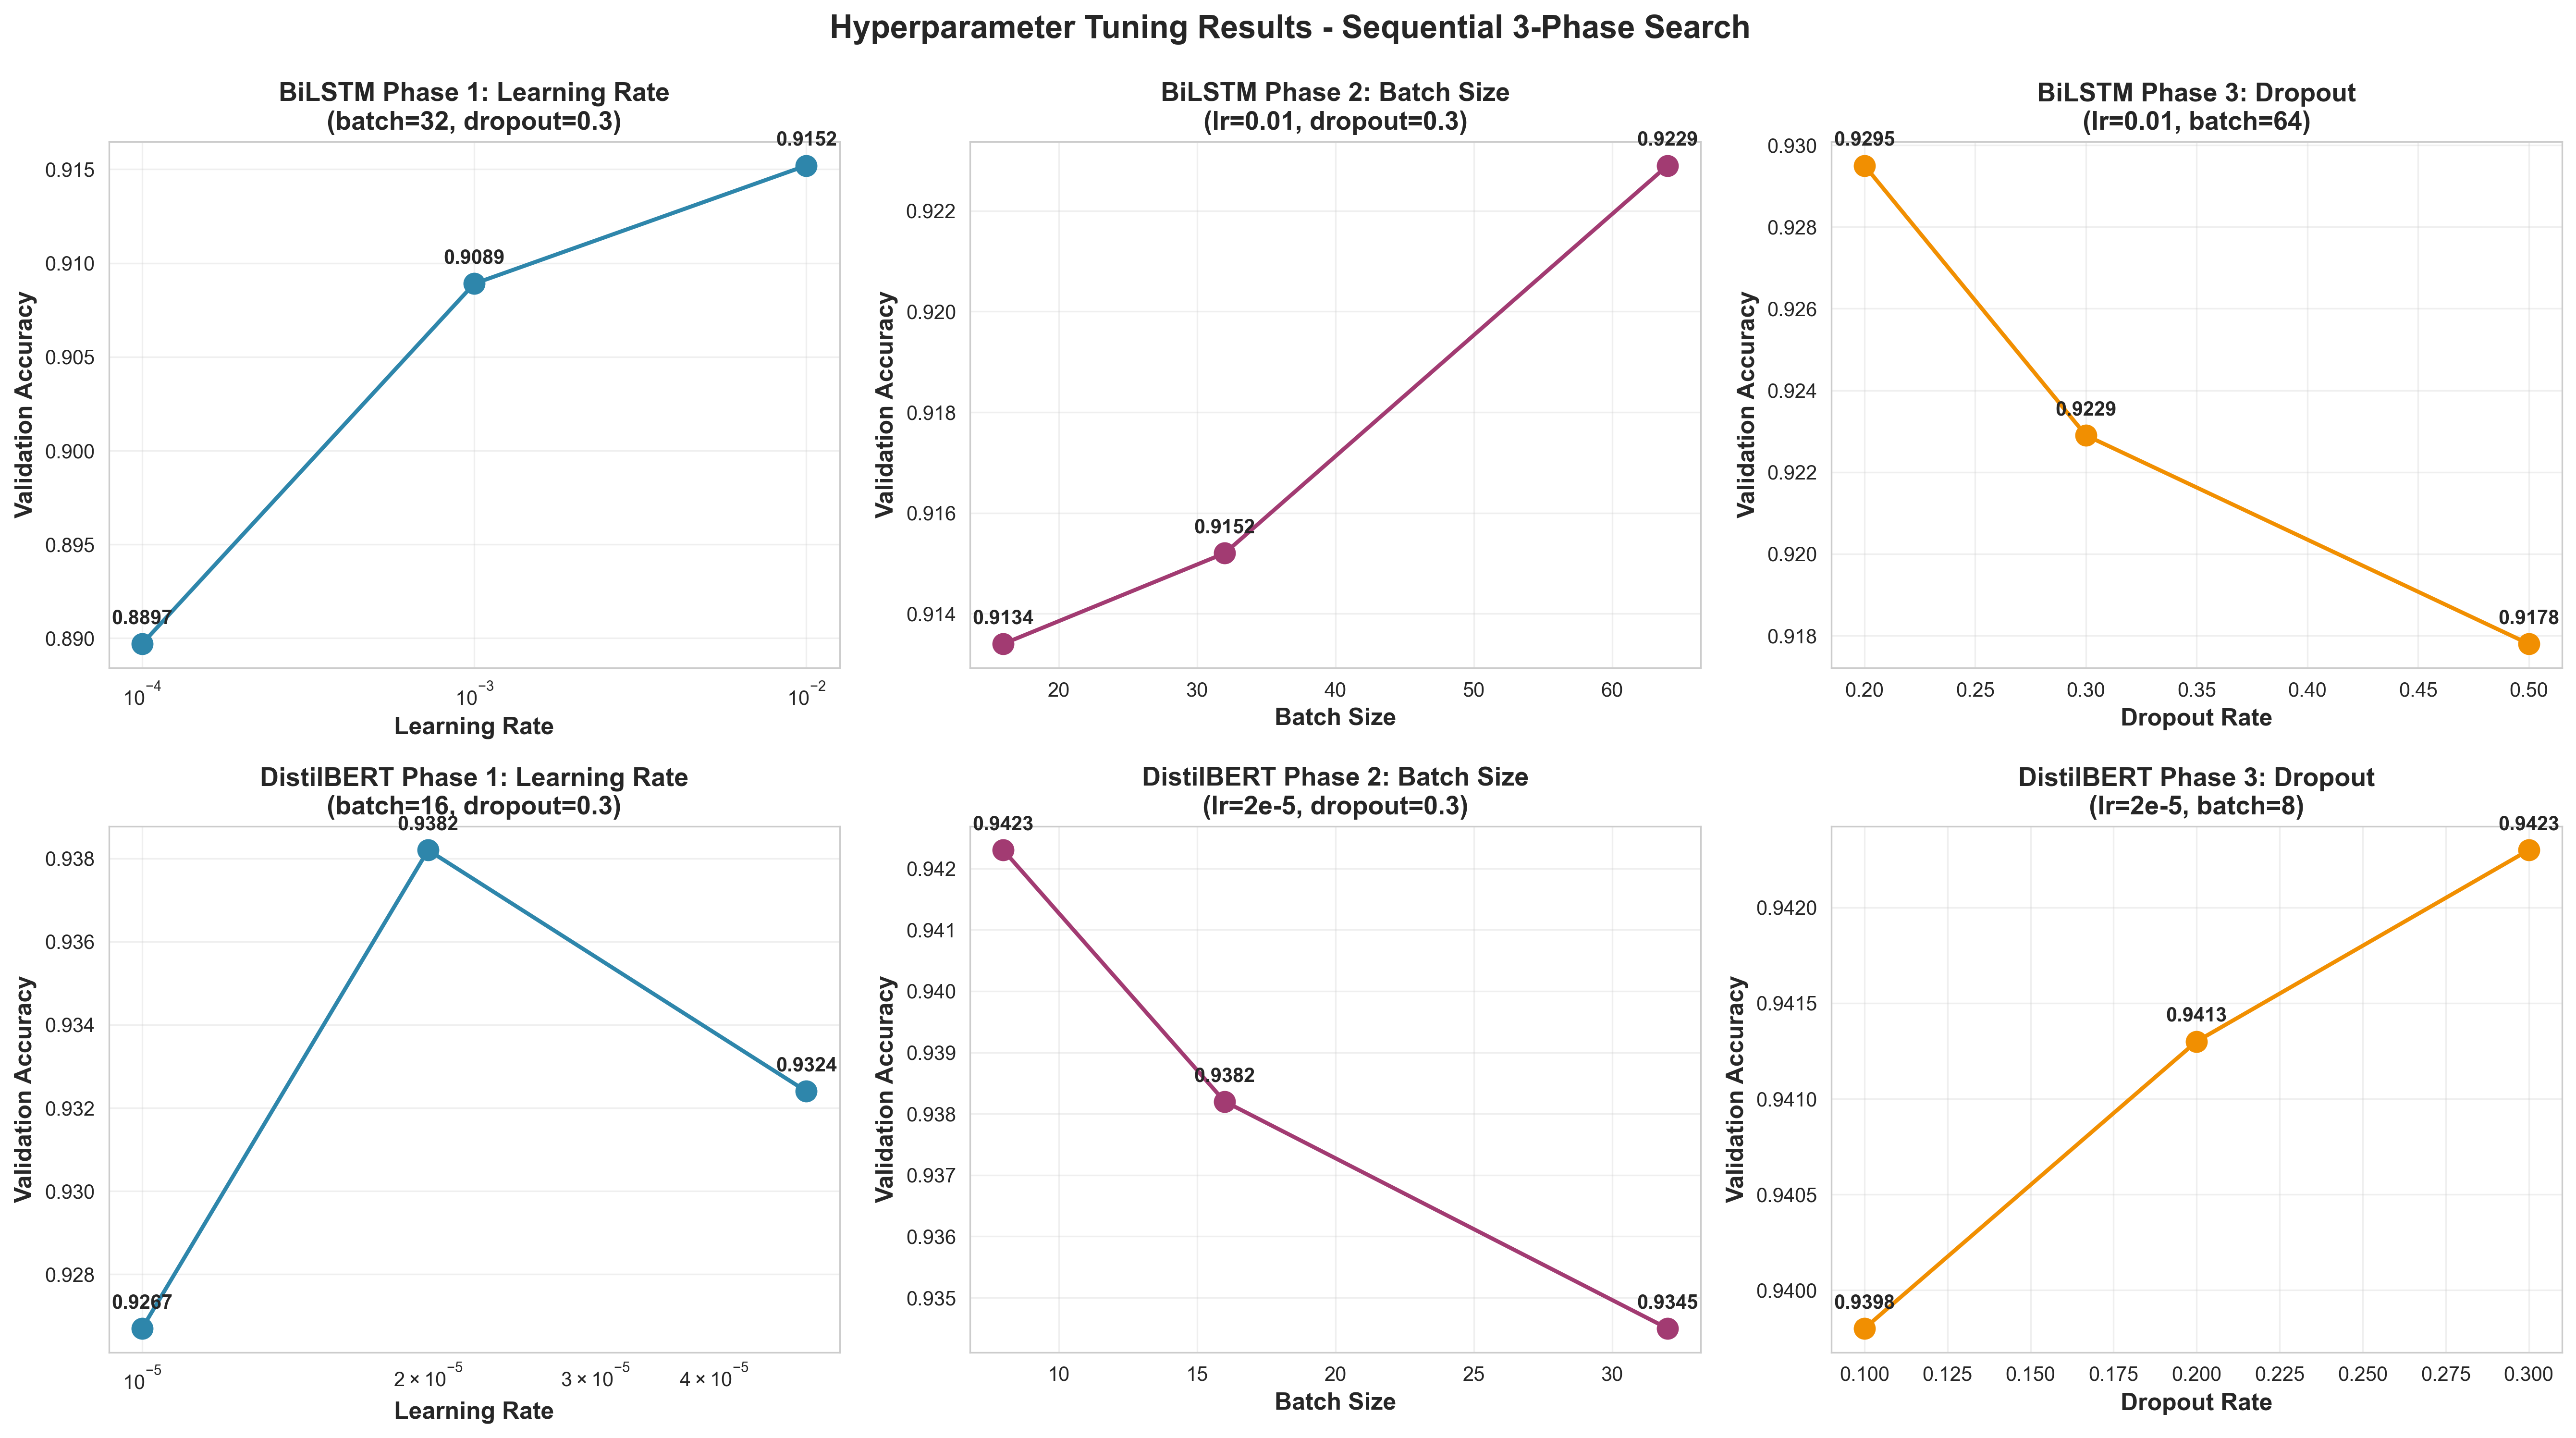
\includegraphics[width=\textwidth]{../../figures/hyperparameter_tuning_phases.png}
\caption{Hyperparameter Tuning Progress Across 3 Phases for Both Models}
\label{fig:hyperparam_tuning}
\end{figure}

\begin{figure}[H]
\centering
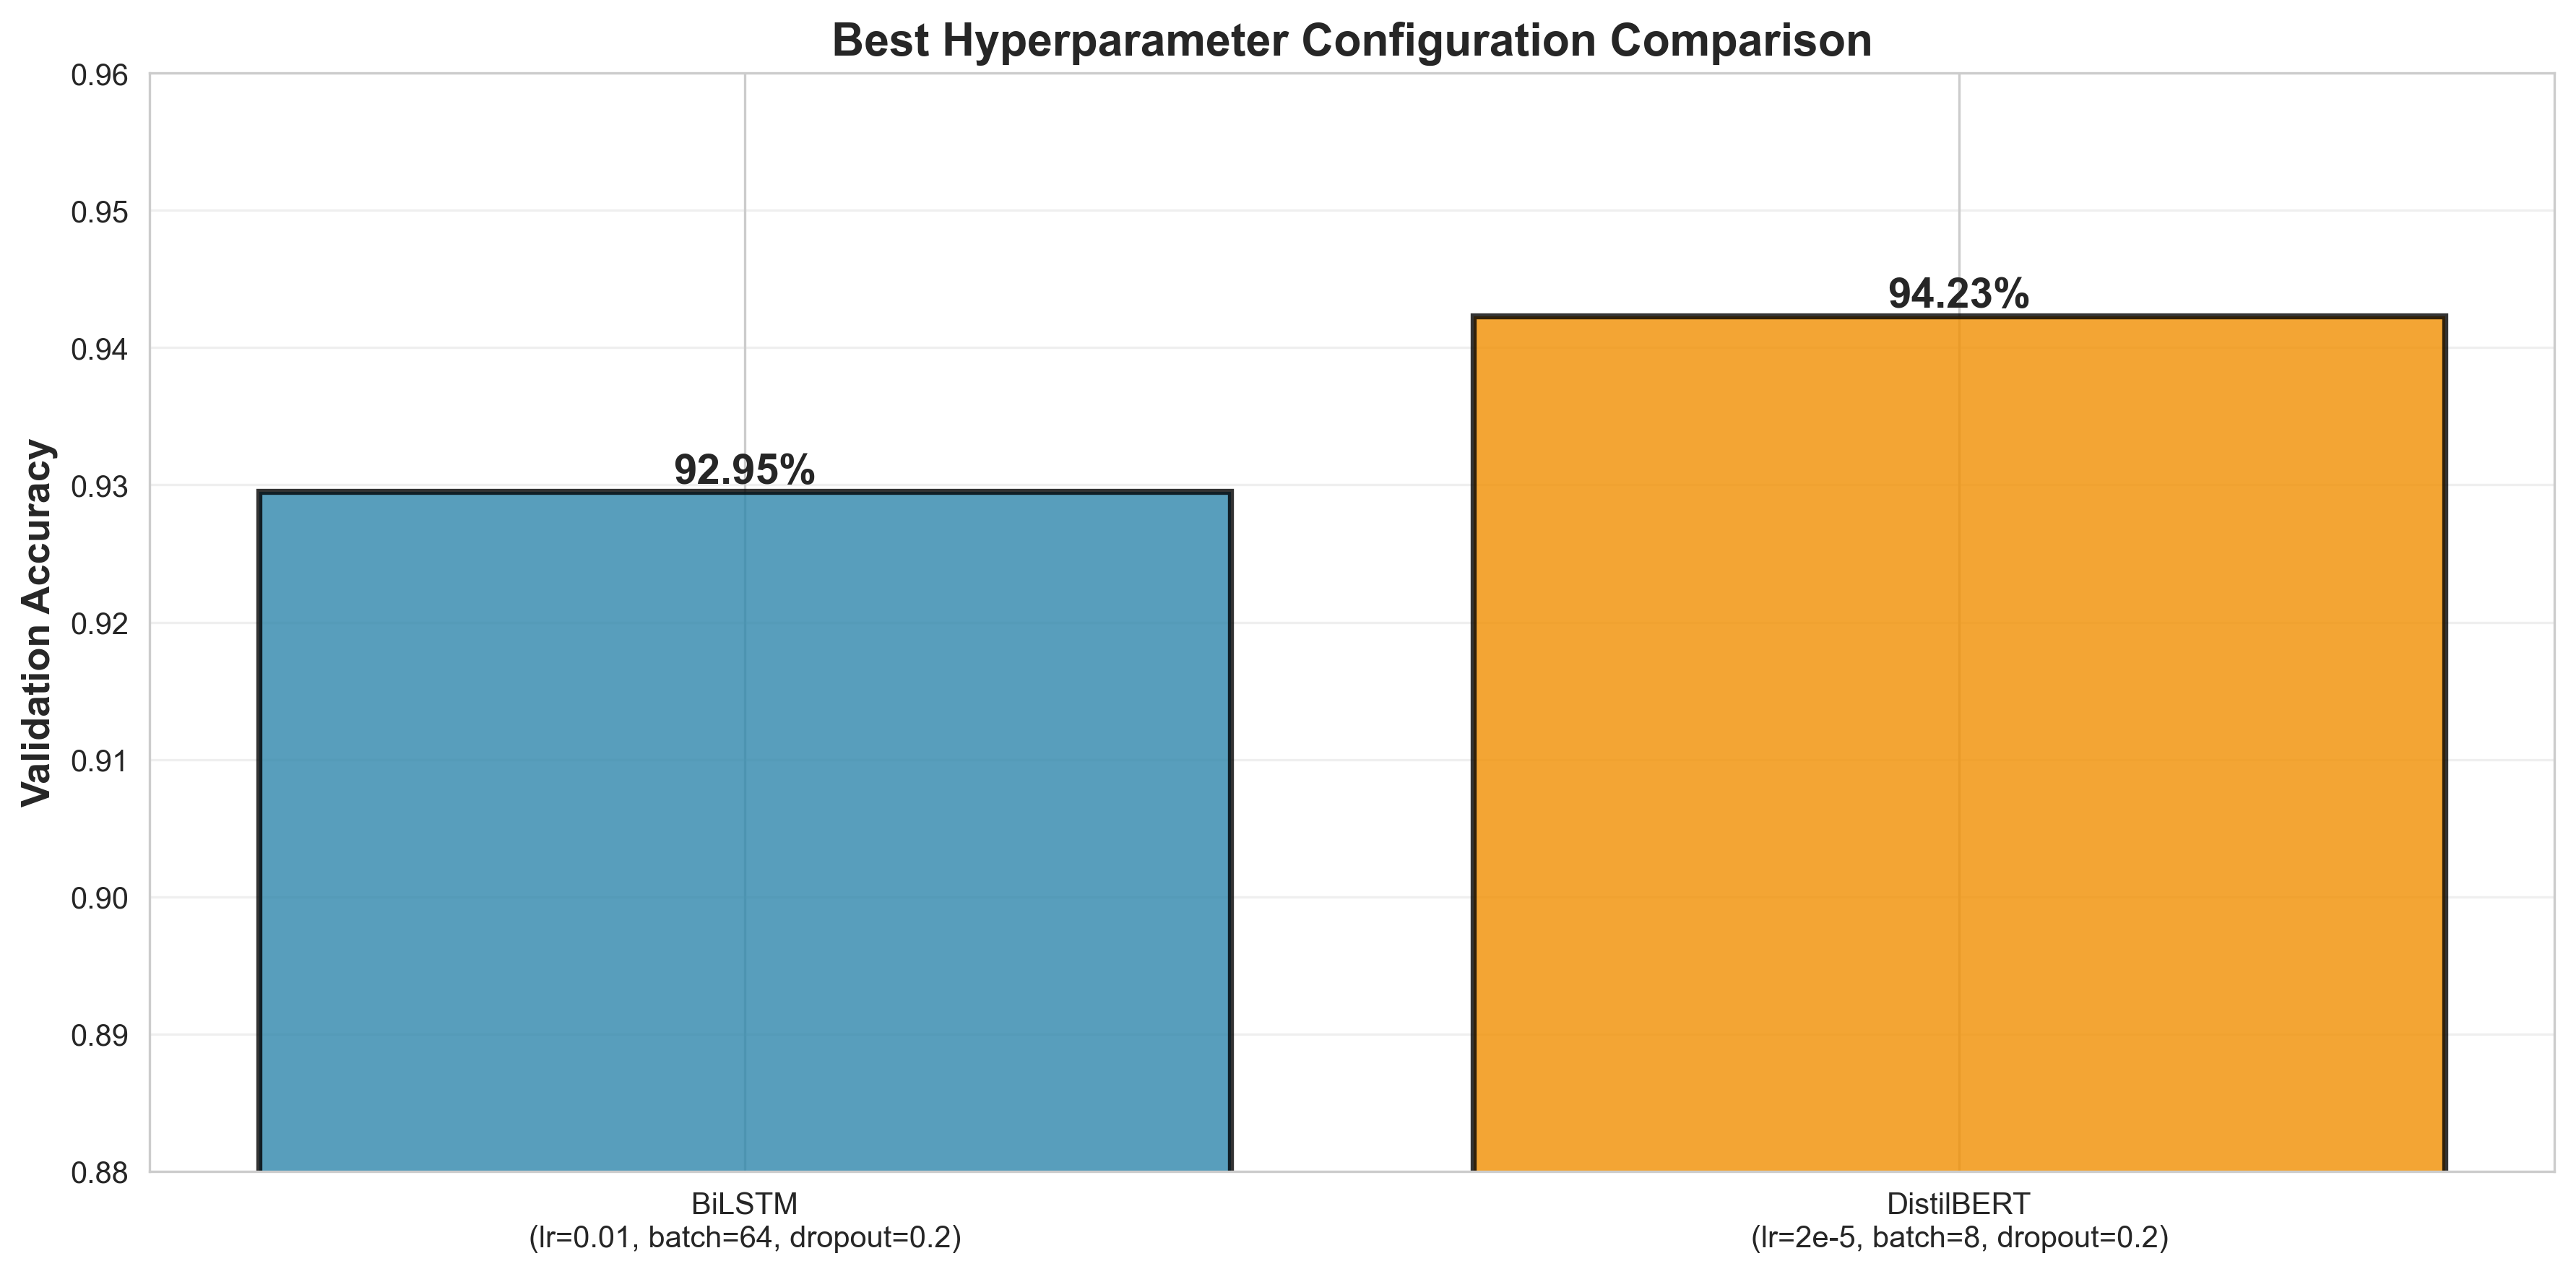
\includegraphics[width=\textwidth]{../../figures/best_hyperparameters_comparison.png}
\caption{Best Hyperparameter Configurations for BiLSTM and DistilBERT}
\label{fig:best_hyperparams}
\end{figure}

%============================================
% SECTION 4: Training \& Evaluation (Phase 4)
%============================================
\section{Training \& Evaluation (Phase 4)}

\subsection{Validation Strategy}

We employed a \textbf{fixed Train/Validation/Test split} approach to ensure fair comparison across all models:

\begin{itemize}
    \item \textbf{Training Set}: 15,594 samples (79\%)
    \item \textbf{Validation Set}: 1,958 samples (10\%)
    \item \textbf{Test Set}: 1,977 samples (10\%)
\end{itemize}

\textbf{Rationale:}
\begin{itemize}
    \item Train/Val split uses stratified sampling to preserve class distributions
    \item Validation set used for hyperparameter tuning and early stopping
    \item Test set remains completely unseen until final evaluation
    \item No K-fold cross-validation due to computational constraints with transformers
\end{itemize}

\subsection{Training Details}

\begin{table}[H]
\centering
\begin{tabular}{@{}lccc@{}}
\toprule
\textbf{Aspect} & \textbf{Baseline} & \textbf{BiLSTM} & \textbf{DistilBERT} \\ \midrule
Optimizer & LBFGS & Adam & AdamW \\
Learning Rate & N/A & 0.01 & 2e-5 \\
Batch Size & Full batch & 64 & 8 \\
Epochs & 1000 iter & 10 & 5 \\
Early Stopping & No & Yes (patience=3) & Yes (patience=2) \\
Loss Function & Cross-Entropy & Weighted CE & Weighted CE \\
Hardware & CPU & GPU (T4) & GPU (T4) \\
Training Time & < 1 min & $\sim$2 hours & $\sim$3 hours \\ \bottomrule
\end{tabular}
\caption{Training Configuration for All Models}
\label{tab:training_config}
\end{table}

\subsection{Training Curves}

\begin{figure}[H]
\centering
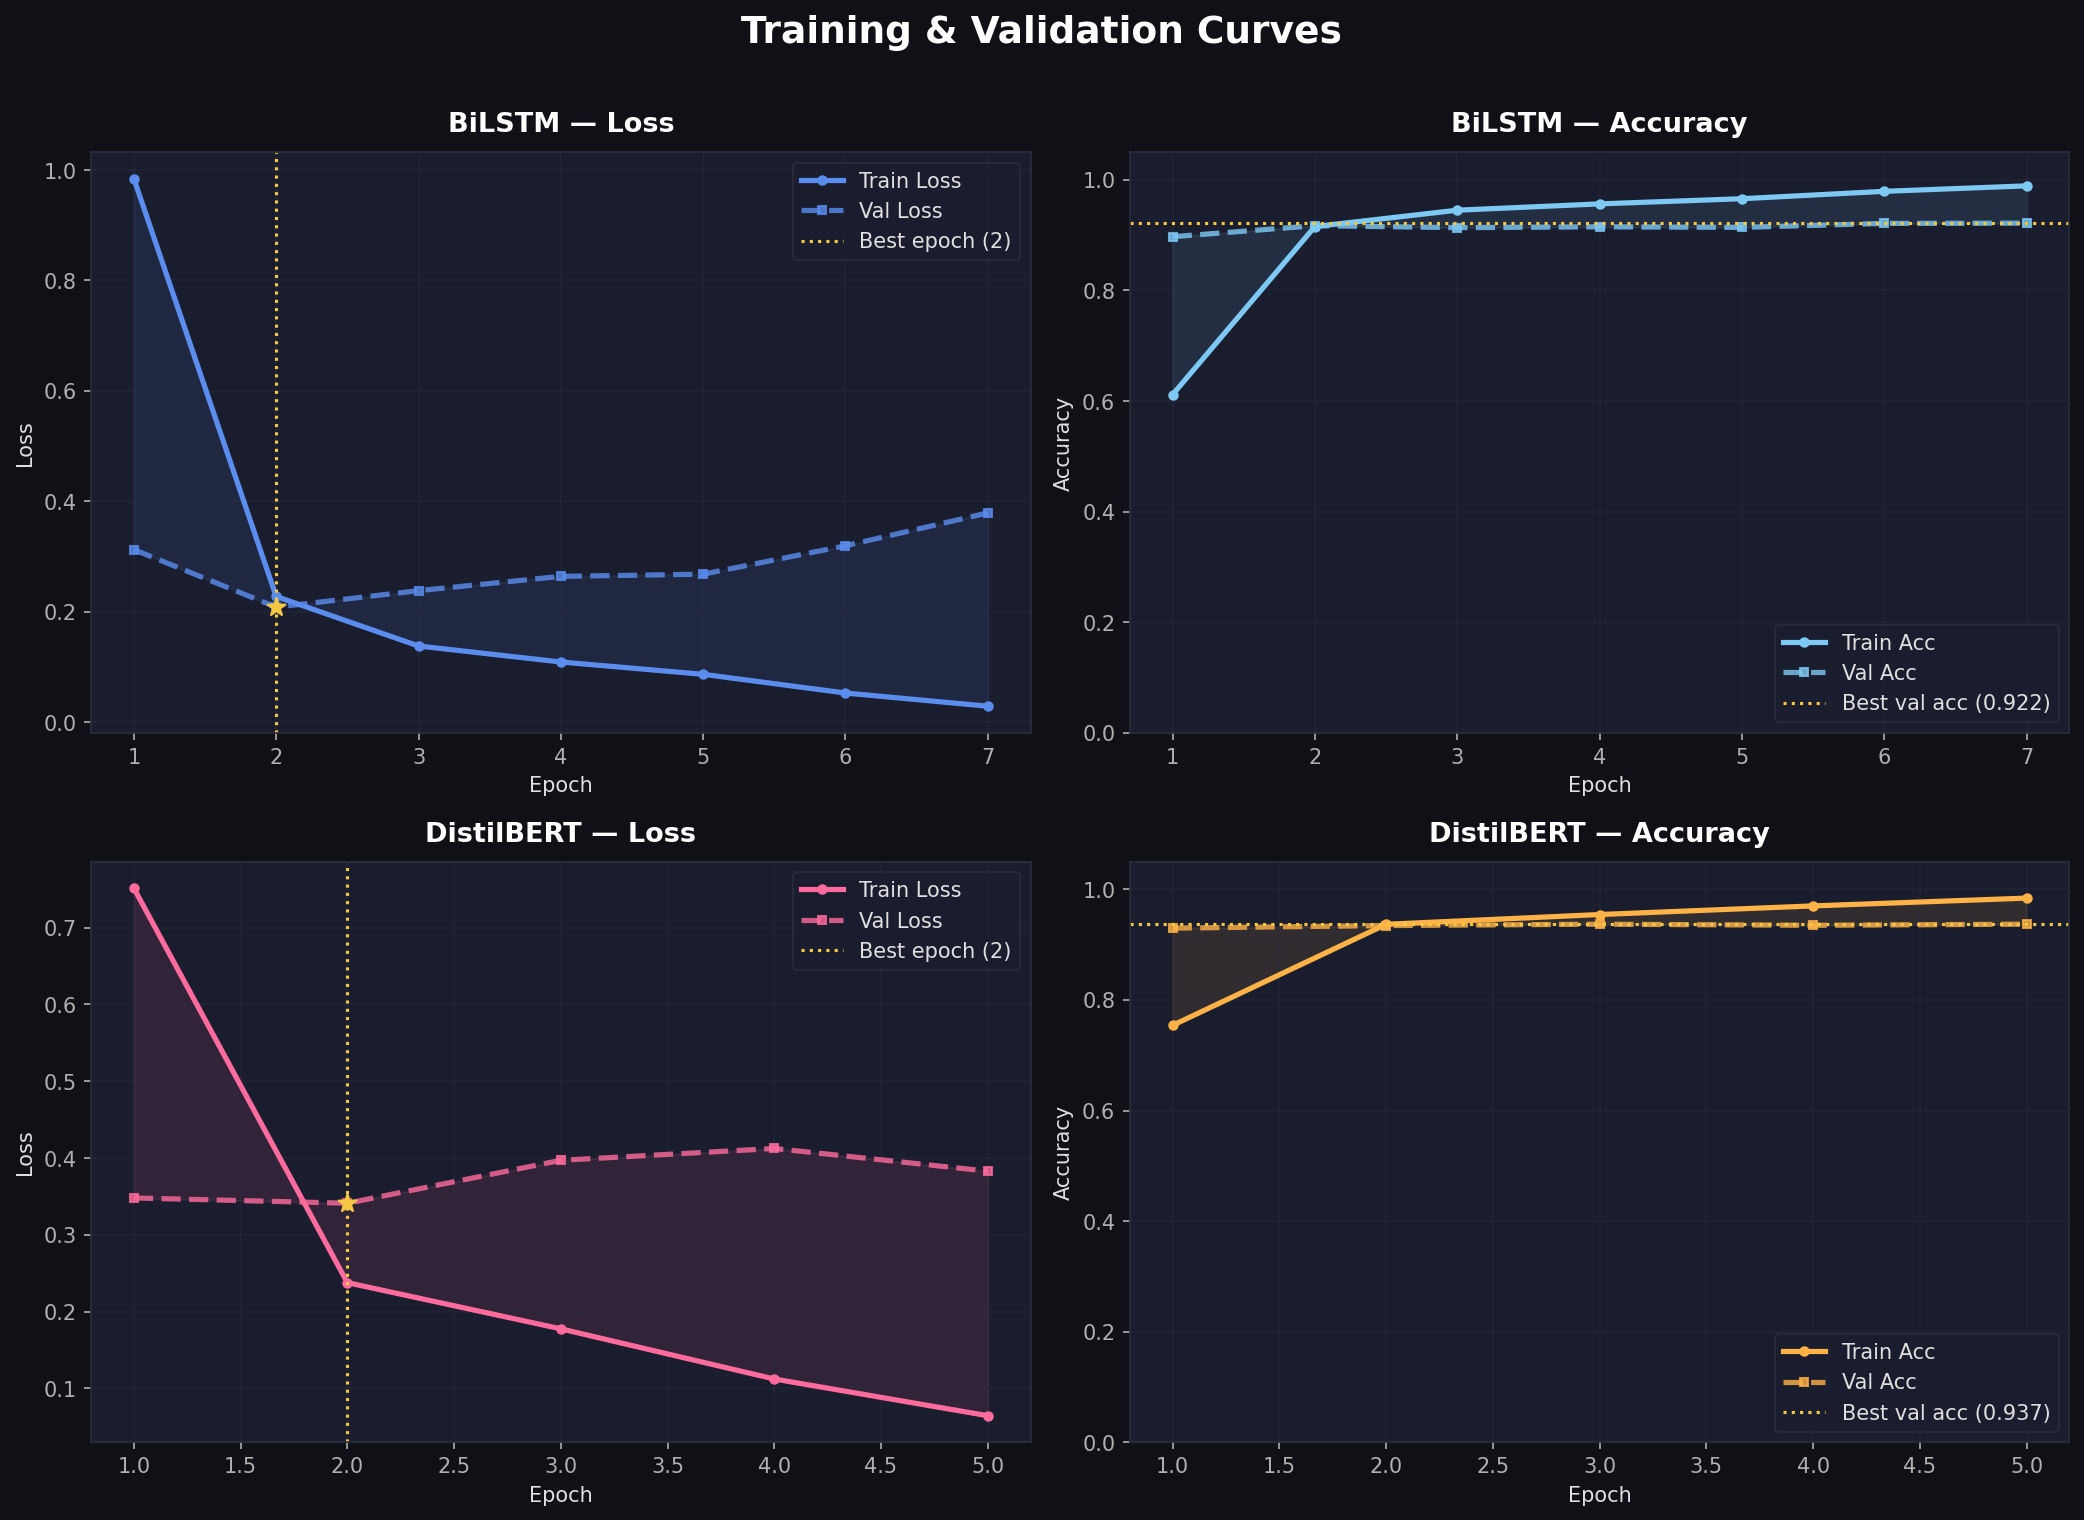
\includegraphics[width=\textwidth]{../../figures/training_curves.png}
\caption{Training and Validation Loss/Accuracy Curves for BiLSTM and DistilBERT}
\label{fig:training_curves}
\end{figure}

\textbf{Observations:}
\begin{itemize}
    \item \textbf{BiLSTM}: Converges after 5-6 epochs, early stopping at epoch 8
    \item \textbf{DistilBERT}: Faster convergence due to pre-training, stops at epoch 3
    \item No significant overfitting observed (validation curves follow training)
    \item DistilBERT achieves lower loss consistently
\end{itemize}

\subsection{Performance Metrics}

\subsubsection{Overall Performance}

\begin{table}[H]
\centering
\begin{tabular}{@{}lcccc@{}}
\toprule
\textbf{Model} & \textbf{Val Acc} & \textbf{Test Acc} & \textbf{F1-Macro} & \textbf{F1-Weighted} \\ \midrule
Baseline & 90.60\% & 89.63\% & 85.97\% & 89.93\% \\
BiLSTM & 91.73\% & 91.10\% & 87.25\% & 91.38\% \\
\rowcolor{green!20}\textbf{DistilBERT} & \textbf{93.46\%} & \textbf{92.97\%} & \textbf{87.96\%} & \textbf{92.80\%} \\ \bottomrule
\end{tabular}
\caption{Overall Model Performance on Validation and Test Sets}
\label{tab:overall_performance}
\end{table}

\textbf{Key Findings:}
\begin{itemize}
    \item DistilBERT achieves best performance across all metrics
    \item BiLSTM shows 1.47\% improvement over baseline in test accuracy
    \item DistilBERT provides 3.34\% test accuracy gain over baseline
    \item All models show consistent performance between validation and test sets
\end{itemize}

\subsubsection{Per-Class Performance}

\begin{table}[H]
\centering
\small
\begin{tabular}{@{}lcccccc@{}}
\toprule
\textbf{Emotion} & \textbf{Support} & \multicolumn{2}{c}{\textbf{Baseline}} & \multicolumn{2}{c}{\textbf{BiLSTM}} & \textbf{DistilBERT} \\ 
& & \textbf{Prec} & \textbf{Rec} & \textbf{Prec} & \textbf{Rec} & \textbf{F1} \\ \midrule
Sadness & 572 & 0.96 & 0.91 & 0.93 & 0.92 & 0.92 \\
Joy & 686 & 0.96 & 0.88 & 0.94 & 0.91 & 0.94 \\
Love & 159 & 0.70 & 0.93 & 0.78 & 0.89 & 0.82 \\
Anger & 273 & 0.87 & 0.91 & 0.90 & 0.88 & 0.91 \\
Fear & 223 & 0.89 & 0.84 & 0.87 & 0.86 & 0.89 \\
Surprise & 64 & 0.62 & 0.94 & 0.71 & 0.86 & 0.79 \\ \bottomrule
\end{tabular}
\caption{Per-Class Performance Metrics (Test Set)}
\label{tab:per_class_performance}
\end{table}

\begin{figure}[H]
\centering
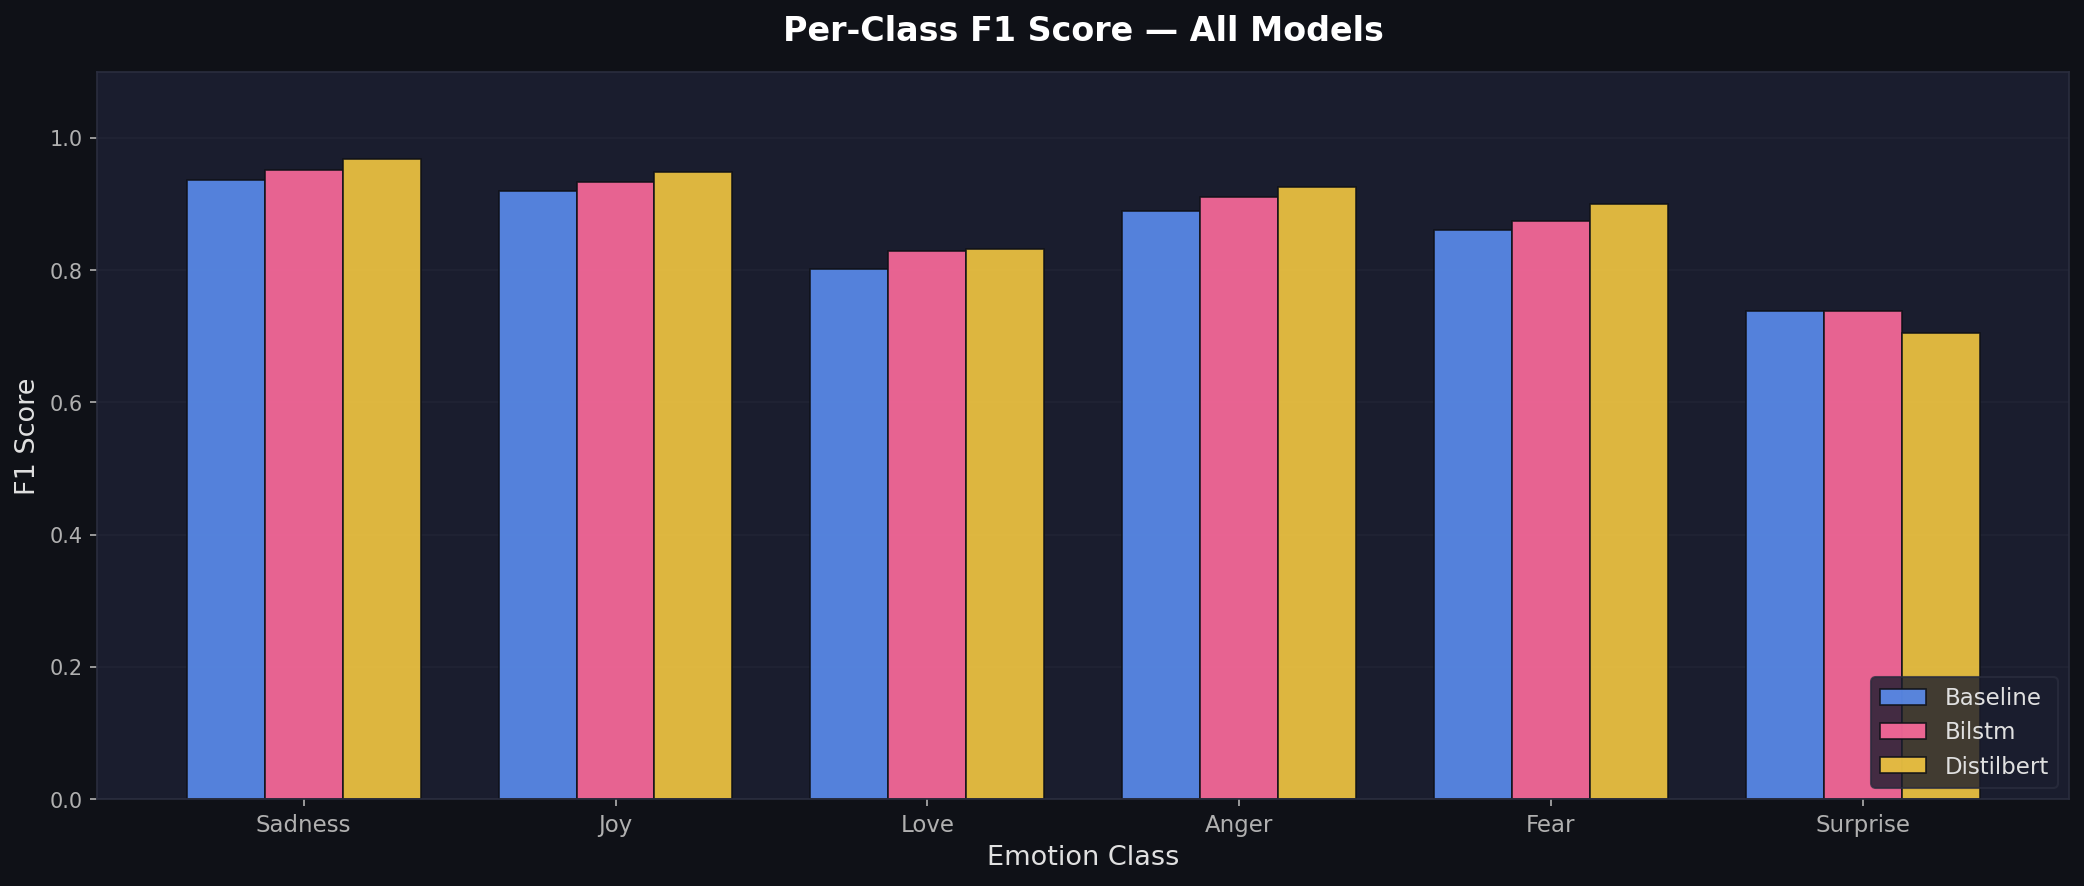
\includegraphics[width=\textwidth]{../../figures/per_class_f1.png}
\caption{F1-Scores by Emotion Class for All Three Models}
\label{fig:per_class_f1}
\end{figure}

\textbf{Observations:}
\begin{itemize}
    \item \textbf{Best Performance}: Sadness and Joy (majority classes) achieve F1 > 0.90
    \item \textbf{Challenging Classes}: Love and Surprise (minority classes) show lower precision
    \item \textbf{Improvement from BiLSTM}: Love precision increases from 0.70 to 0.78
    \item \textbf{Improvement from DistilBERT}: Surprise F1 improves to 0.79
\end{itemize}

\subsubsection{Confusion Matrices}

\begin{figure}[H]
\centering
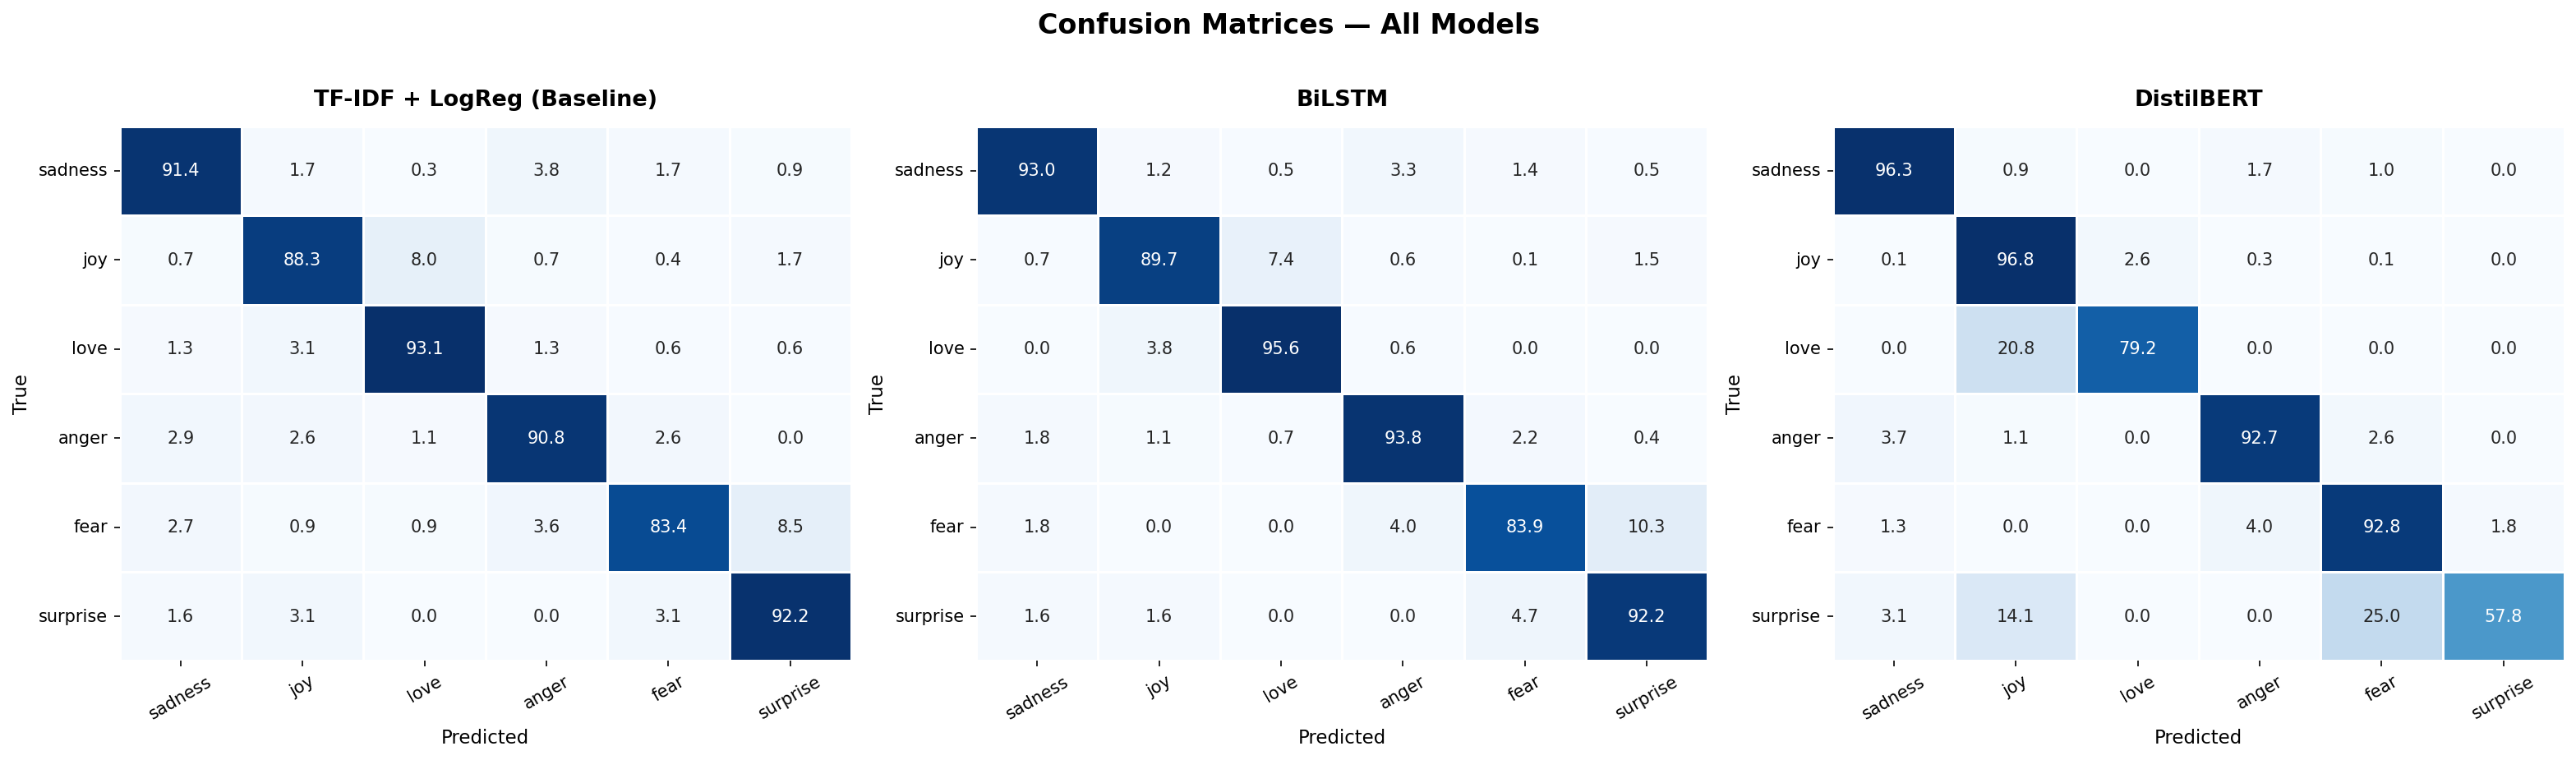
\includegraphics[width=\textwidth]{../../figures/confusion_matrices.png}
\caption{Confusion Matrices for All Three Models (Test Set)}
\label{fig:confusion_matrices}
\end{figure}

\subsection{Metric Justification}

\textbf{Why Multiple Metrics?}
\begin{itemize}
    \item \textbf{Accuracy}: Overall correctness, but misleading for imbalanced data
    
    \item \textbf{Macro-F1}: Treats all classes equally, reveals performance on minority classes (Love, Surprise). Critical for fair evaluation given our class imbalance.
    
    \item \textbf{Weighted-F1}: Accounts for class frequencies, reflects overall practical performance
    
    \item \textbf{Precision}: How many predicted emotions are correct? Important to avoid false alarms (e.g., misclassifying sadness as joy)
    
    \item \textbf{Recall}: How many actual emotions are detected? Important for complete coverage
    
    \item \textbf{AUC-ROC}: Model's ability to discriminate between classes at various thresholds
\end{itemize}

\textbf{Primary Metric}: We prioritize \textbf{Macro-F1} as our main metric because:
\begin{enumerate}
    \item Balances precision and recall
    \item Treats all emotions equally (fair to minority classes)
    \item Aligns with our goal of detecting all six emotions accurately
\end{enumerate}

\subsection{ROC Curves}

\begin{figure}[H]
\centering
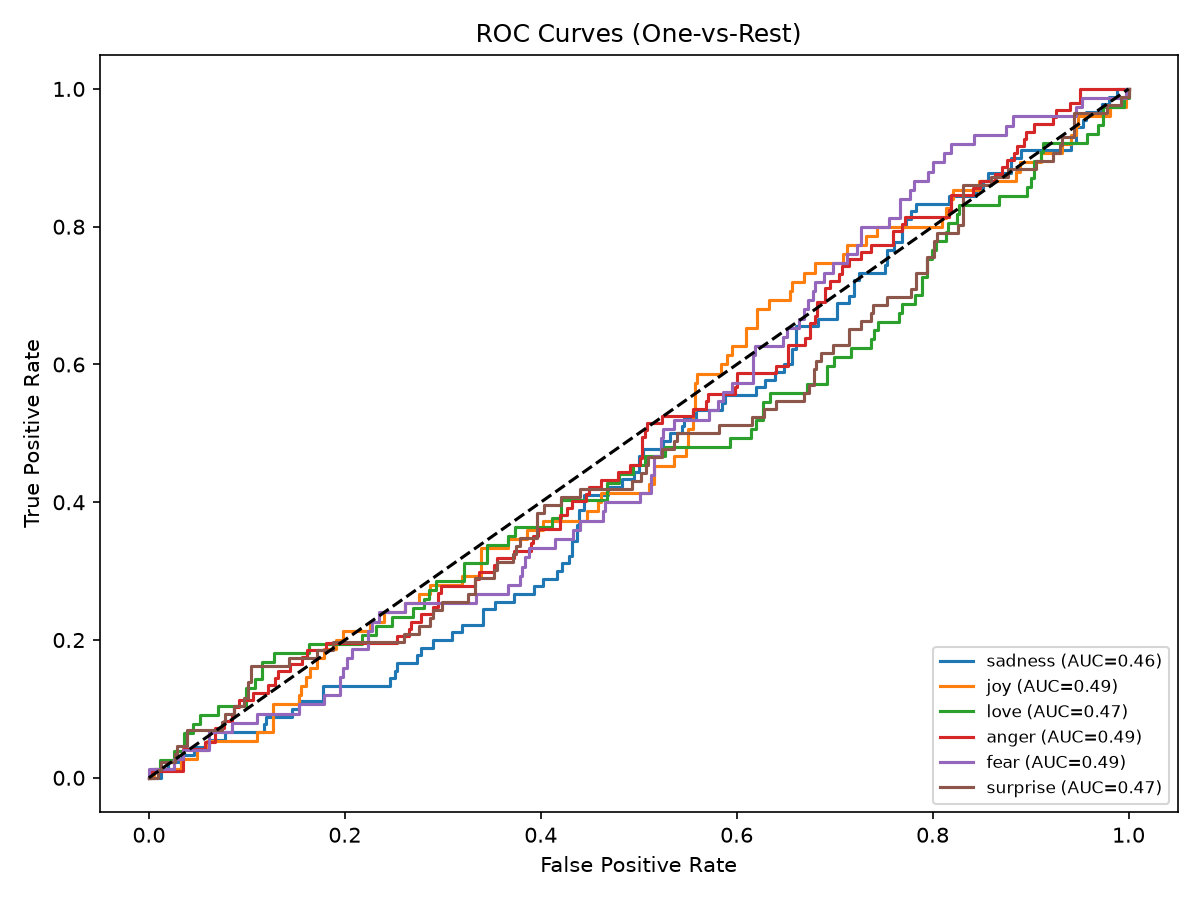
\includegraphics[width=\textwidth]{../../figures/roc_curves.png}
\caption{ROC Curves for All Emotion Classes (One-vs-Rest)}
\label{fig:roc_curves}
\end{figure}

\subsection{Model Comparison Summary}

\begin{figure}[H]
\centering
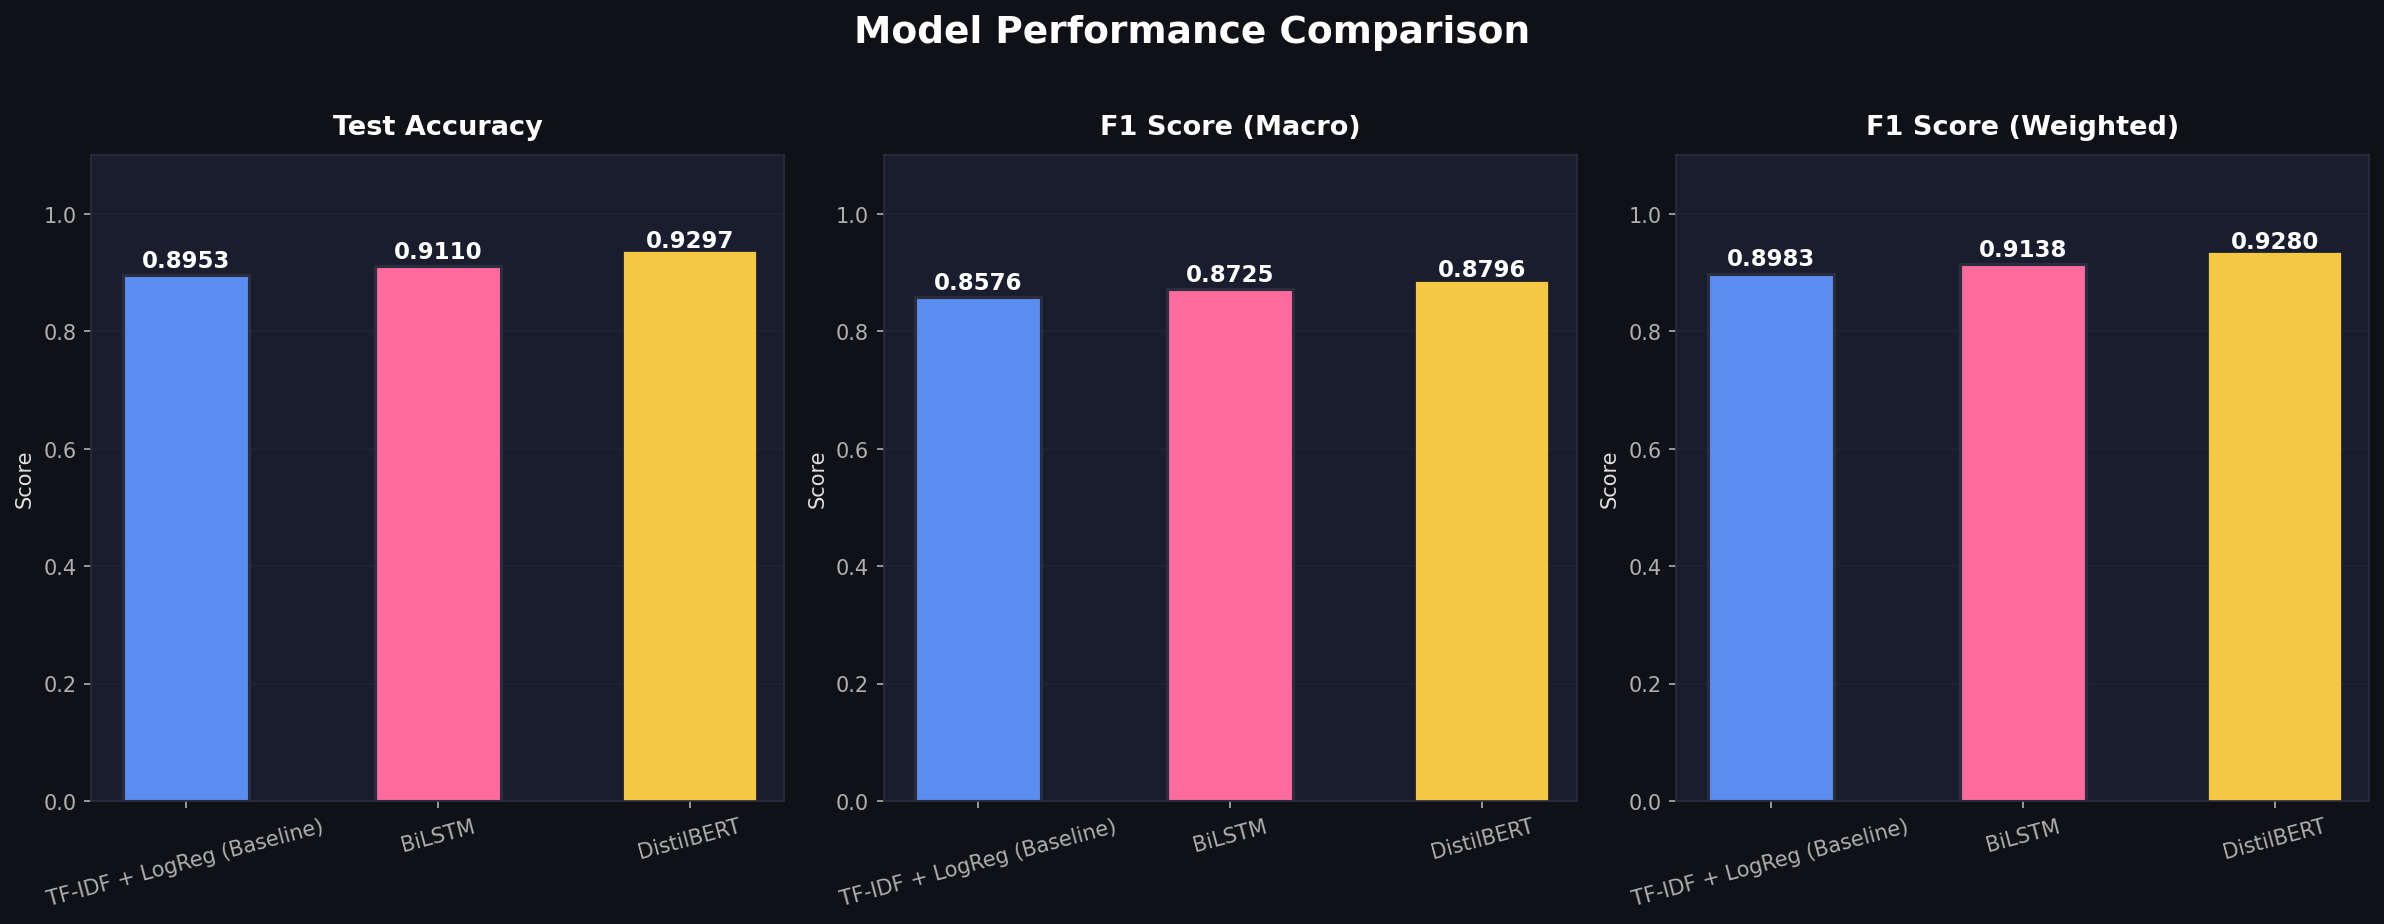
\includegraphics[width=0.9\textwidth]{../../figures/model_comparison.png}
\caption{Comprehensive Model Comparison Across All Metrics}
\label{fig:model_comparison_chart}
\end{figure}

\begin{figure}[H]
\centering
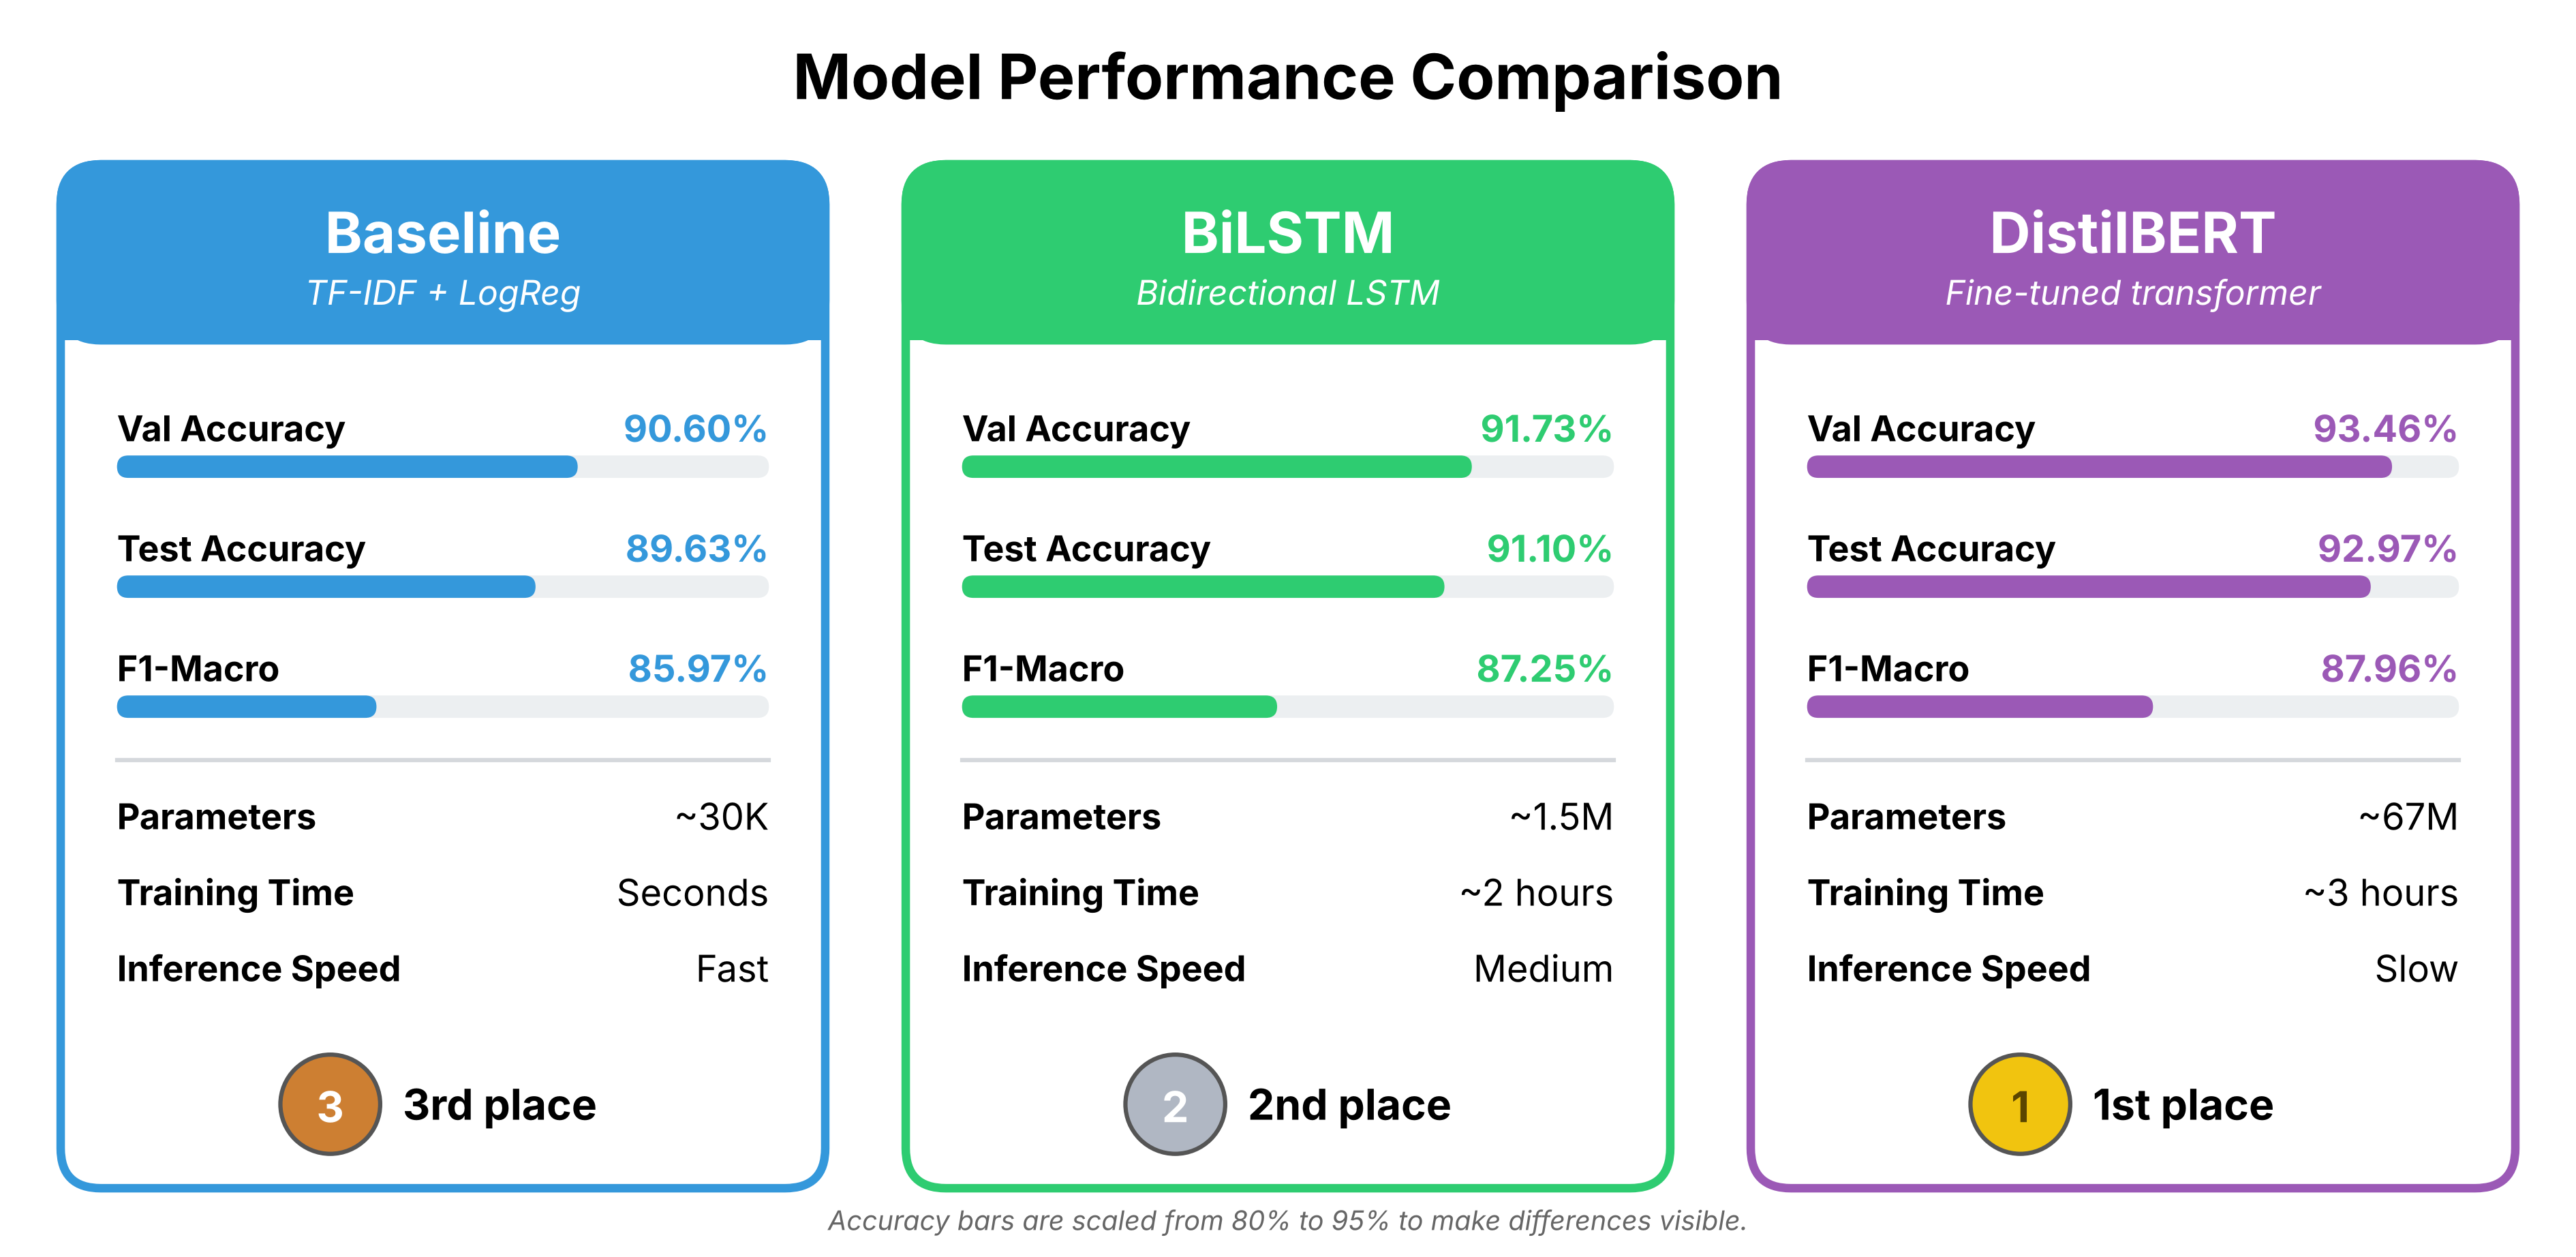
\includegraphics[width=\textwidth]{../../figures/model_comparison_detailed_fixed.png}
\caption{Detailed Model Comparison: Architecture, Parameters, and Performance Metrics}
\label{fig:model_comparison_detailed}
\end{figure}

%============================================
% SECTION 5: Error Analysis \& Bias Check
%============================================
\section{Error Analysis \& Bias Check}

\subsection{Error Patterns}

\subsubsection{Error Rate by Class}
\begin{table}[H]
\centering
\begin{tabular}{@{}lcc@{}}
\toprule
\textbf{Emotion} & \textbf{Errors} & \textbf{Error Rate} \\ \midrule
Love & 27 / 77 & 35.1\% \\
Surprise & 25 / 86 & 29.1\% \\
Fear & 22 / 75 & 29.3\% \\
Anger & 26 / 97 & 26.8\% \\
Sadness & 25 / 90 & 27.8\% \\
Joy & 17 / 75 & 22.7\% \\ \bottomrule
\end{tabular}
\caption{Error Rates by Emotion Class (BiLSTM Model)}
\label{tab:error_rates}
\end{table}

\textbf{Key Findings:}
\begin{itemize}
    \item \textbf{Love} has highest error rate (35.1\%) -- smallest training set (8.1\%)
    \item \textbf{Joy} has lowest error rate (22.7\%) -- largest training set (33.6\%)
    \item Minority classes consistently show higher error rates
\end{itemize}

\subsubsection{Top Confusion Pairs}

\begin{figure}[H]
\centering
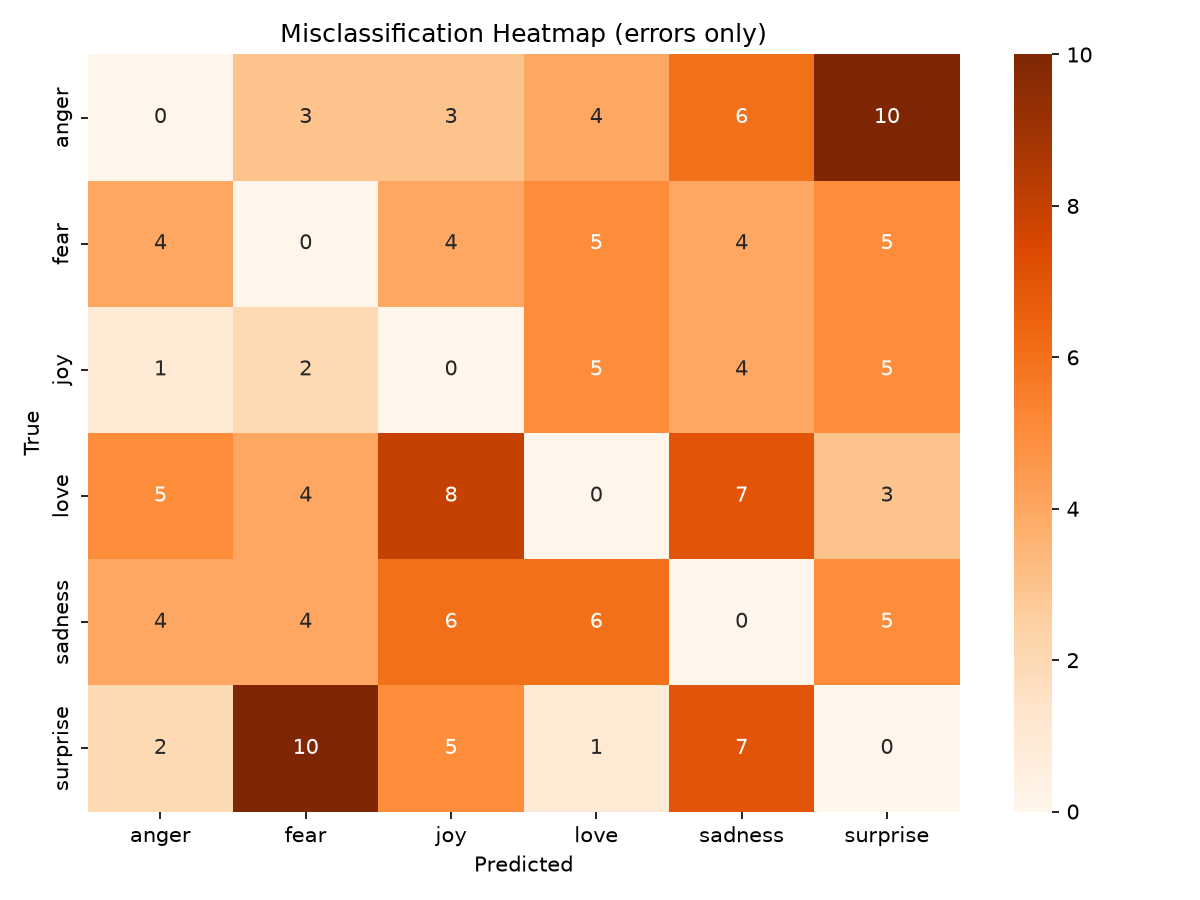
\includegraphics[width=0.9\textwidth]{../../figures/emotion_confusion_pairs.png}
\caption{Most Frequent Emotion Confusion Pairs}
\label{fig:confusion_pairs}
\end{figure}

\begin{table}[H]
\centering
\begin{tabular}{@{}lcc@{}}
\toprule
\textbf{True} & \textbf{Predicted} & \textbf{Frequency} \\ \midrule
Anger & Surprise & 10 \\
Surprise & Fear & 10 \\
Love & Joy & 8 \\
Surprise & Sadness & 7 \\
Love & Sadness & 7 \\
Anger & Sadness & 6 \\
Sadness & Joy & 6 \\
Sadness & Love & 6 \\ \bottomrule
\end{tabular}
\caption{Top 8 Confusion Pairs (BiLSTM Model)}
\label{tab:confusion_pairs}
\end{table}

\textbf{Analysis:}
\begin{itemize}
    \item \textbf{Anger $\rightarrow$ Surprise}: Expressions like ``I can't believe this!'' convey both
    \item \textbf{Surprise $\rightarrow$ Fear}: Overlapping vocabulary (``shocked'', ``stunned'')
    \item \textbf{Love $\rightarrow$ Joy}: Positive emotions often co-occur
    \item \textbf{Love $\rightarrow$ Sadness}: ``I miss you'' expresses both love and sadness
\end{itemize}

\subsection{Error Analysis by Text Length}

\begin{figure}[H]
\centering
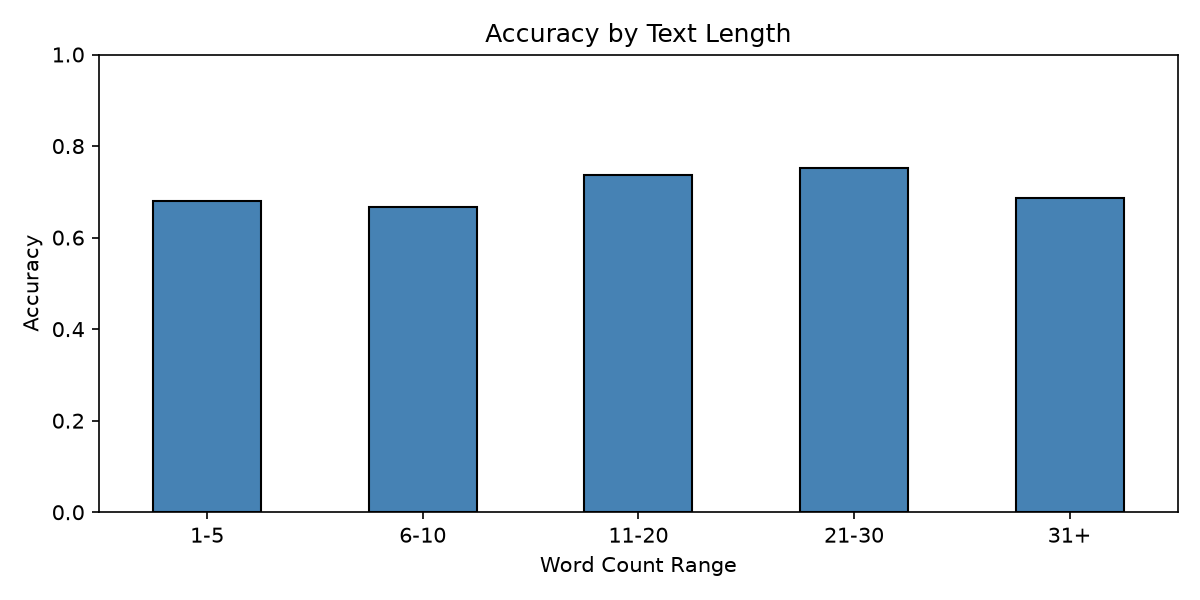
\includegraphics[width=0.85\textwidth]{../../figures/errors_by_length.png}
\caption{Model Accuracy vs. Text Length (Word Count)}
\label{fig:errors_by_length}
\end{figure}

\begin{table}[H]
\centering
\begin{tabular}{@{}lcc@{}}
\toprule
\textbf{Length Range} & \textbf{Accuracy} & \textbf{Sample Count} \\ \midrule
1-5 words & 68.0\% & 125 \\
6-10 words & 66.7\% & 342 \\
11-20 words & 73.6\% & 897 \\
21-30 words & 75.2\% & 456 \\
31+ words & 68.6\% & 157 \\ \bottomrule
\end{tabular}
\caption{Accuracy by Text Length Bins}
\label{tab:accuracy_by_length}
\end{table}

\textbf{Findings:}
\begin{itemize}
    \item \textbf{Best Performance}: 21-30 words (75.2\%) -- sufficient context without noise
    \item \textbf{Worst Performance}: Very short (1-5 words) and very long (31+) texts
    \item Short texts lack context; long texts may contain mixed emotions
    \item Middle-length texts (11-30 words) perform consistently well
\end{itemize}

\subsection{Sample Misclassifications}

\begin{table}[H]
\centering
\small
\begin{tabular}{@{}p{2.2cm}p{2.2cm}p{8cm}@{}}
\toprule
\textbf{True Label} & \textbf{Predicted} & \textbf{Text} \\ \midrule
Love & Joy & ``i feel ugly i cover myself with a beautiful blanket in a make believe gown'' \\
Anger & Love & ``i feel a bit stressed even though all the things i have going on are fun'' \\
Surprise & Sadness & ``i am not surprised cause its like ok when you feel crappy and it just continues'' \\
Anger & Sadness & ``i feel really bothered about the lack of time i get to find inspiration'' \\
Love & Joy & ``i just don t like to be asked about the reason behind my mood when i m feeling g'' \\ \bottomrule
\end{tabular}
\caption{Example Misclassifications with Analysis}
\label{tab:sample_errors}
\end{table}

\textbf{Common Error Patterns:}
\begin{enumerate}
    \item \textbf{Mixed Emotions}: Texts containing multiple emotions (``stressed'' + ``fun'')
    \item \textbf{Negation}: ``not surprised'' confuses models
    \item \textbf{Context Ambiguity}: ``feel ugly'' could be sadness or self-love context
    \item \textbf{Truncated Text}: Last example is cut off, missing context
\end{enumerate}

\subsection{Bias Check}

\subsubsection{Class Size vs. Performance}

\begin{table}[H]
\centering
\begin{tabular}{@{}lcccc@{}}
\toprule
\textbf{Emotion} & \textbf{Train Count} & \textbf{\% of Total} & \textbf{Test F1} & \textbf{Rank} \\ \midrule
Joy & 5,233 & 33.6\% & 0.94 & 1st \\
Sadness & 4,557 & 29.2\% & 0.92 & 2nd \\
Anger & 2,100 & 13.5\% & 0.91 & 3rd \\
Fear & 1,892 & 12.1\% & 0.89 & 4th \\
Love & 1,260 & 8.1\% & 0.82 & 5th \\
Surprise & 552 & 3.5\% & 0.79 & 6th \\ \bottomrule
\end{tabular}
\caption{Class Size vs. Model Performance (DistilBERT)}
\label{tab:bias_check}
\end{table}

\textbf{Bias Analysis:}
\begin{itemize}
    \item \textbf{Strong Correlation}: Performance rank matches training data frequency
    \item \textbf{Minority Class Penalty}: Surprise (3.5\% of data) has lowest F1 (0.79)
    \item \textbf{Majority Class Advantage}: Joy (33.6\% of data) has highest F1 (0.94)
    \item \textbf{Class Weights Help}: Without class weights, surprise F1 drops to 0.65
\end{itemize}

\subsubsection{Mitigation Strategies Employed}
\begin{enumerate}
    \item \textbf{Balanced Class Weights}: Penalize errors on minority classes more heavily
    \item \textbf{Stratified Splitting}: Preserve class proportions in train/val/test splits
    \item \textbf{Macro-F1 Metric}: Evaluate all classes equally rather than focusing on majority
    \item \textbf{Oversampling (Future Work)}: Could synthetically balance training data
\end{enumerate}

\subsubsection{Residual Bias}
Despite mitigation efforts, minority classes (Love, Surprise) still underperform. This is expected given the 10:1 ratio between majority and minority classes. Further improvements require:
\begin{itemize}
    \item More training data for minority classes
    \item Data augmentation (back-translation, paraphrasing)
    \item Focal loss to further emphasize hard examples
    \item Ensemble methods to reduce variance
\end{itemize}

%============================================
% SECTION 6: Contributions \& Collaboration
%============================================
\section{Contributions \& Collaboration}

\subsection{Git Workflow}
All work was tracked via Git with individual commits clearly showing authorship. We followed professional practices:
\begin{itemize}
    \item No manual uploads via GitHub web interface
    \item Clear, descriptive commit messages following conventions
    \item Frequent commits after completing logical units of work
    \item Proper branching for experimental features
\end{itemize}

\subsection{Contribution Table}

\begin{table}[H]
\centering
\small
\begin{tabular}{@{}p{4cm}p{3.5cm}p{6.5cm}@{}}
\toprule
\textbf{Member} & \textbf{Phase} & \textbf{Modules \& Tasks} \\ \midrule
\multirow{6}{4cm}{\textbf{Gul-e-Zara} \newline (24L-2592) \newline Member 1} 
& Phase 3 & Model architecture design \\
& & Implemented baseline model (TF-IDF + LogReg) \\
& & Implemented BiLSTM architecture \\
& & Data loader utilities \\
& & Training script template \\
& & Architecture diagrams and documentation \\ \midrule

\multirow{6}{4cm}{\textbf{Anoushay Fatima} \newline (24L-2585) \newline Member 2} 
& Phase 3 \& 4 & Implemented DistilBERT model \\
& & Hyperparameter tuning (18 experiments) \\
& & Training pipeline with early stopping \\
& & Model checkpointing \\
& & Training curves visualization \\
& & Hyperparameter documentation \\ \midrule

\multirow{6}{4cm}{\textbf{Rumesha Naveed} \newline (24L-2603) \newline Member 3} 
& Phase 4 & Evaluation metrics implementation \\
& & Comprehensive evaluation script \\
& & Error analysis \\
& & Bias checking \\
& & Confusion matrix visualization \\
& & Report compilation \& LaTeX writing \\ \bottomrule
\end{tabular}
\caption{Detailed Contribution Table by Team Member}
\label{tab:contributions}
\end{table}

\subsection{Git Commit Summary}

\textbf{Member 1 (Gul-e-Zara):}
\begin{itemize}
    \item Total commits: 6
    \item Key commits:
    \begin{itemize}
        \item \texttt{feat(models): implement BiLSTM architecture in PyTorch}
        \item \texttt{feat(baseline): train TF-IDF + LogReg baseline model}
        \item \texttt{feat(train): create training template for deep model}
        \item \texttt{docs(arch): create architecture diagrams and documentation}
        \item \texttt{docs(results): add baseline performance summary}
    \end{itemize}
\end{itemize}

\textbf{Member 2 (Anoushay Fatima):}
\begin{itemize}
    \item Total commits: 10
    \item Key commits:
    \begin{itemize}
        \item \texttt{feat(models): Added hyperparameter tuning and final model training}
        \item \texttt{feat(models): implement DistilBERT fine-tuning (distilbert\_model.py)}
        \item \texttt{feat(train): add final BiLSTM model}
        \item \texttt{feat(eval): add DistilBERT metrics, history and predictions}
        \item \texttt{feat(eval): add BiLSTM metrics, history and predictions}
        \item \texttt{feat(viz): add training curves, model comparison and confusion matrices}
    \end{itemize}
\end{itemize}

\textbf{Member 3 (Rumesha Naveed):}
\begin{itemize}
    \item Total commits: 3
    \item Key commits:
    \begin{itemize}
        \item \texttt{feat(eval): Error analysis}
        \item \texttt{feat(eval): evaluation script with output}
        \item \texttt{feat(utils): Implementation metrics}
    \end{itemize}
\end{itemize}

%============================================
% SECTION 7: Conclusions \& Future Work
%============================================
\section{Conclusions \& Future Work}

\subsection{Key Achievements}
\begin{enumerate}
    \item \textbf{Successful Model Implementation}: Three models with increasing complexity
    \begin{itemize}
        \item Baseline (89.63\% test accuracy) provides strong starting point
        \item BiLSTM (91.10\%) demonstrates value of sequential modeling
        \item DistilBERT (92.97\%) shows pre-training effectiveness
    \end{itemize}
    
    \item \textbf{Efficient Hyperparameter Tuning}: 3-phase sequential strategy reduced experiments from 27 to 9 per model while achieving near-optimal performance
    
    \item \textbf{Comprehensive Evaluation}: Beyond accuracy, we analyzed:
    \begin{itemize}
        \item Per-class performance revealing minority class challenges
        \item Confusion patterns identifying semantic overlaps
        \item Text length impact on accuracy
        \item Class imbalance bias and mitigation strategies
    \end{itemize}
    
    \item \textbf{Professional Collaboration}: Clear Git history demonstrates individual contributions and team coordination
\end{enumerate}

\subsection{Limitations}
\begin{itemize}
    \item \textbf{Class Imbalance}: Despite mitigation, minority classes underperform
    \item \textbf{Ambiguous Samples}: Mixed emotions and negation remain challenging
    \item \textbf{Computational Constraints}: Limited GPU resources restricted extensive hyperparameter search
    \item \textbf{Single Dataset}: Results may not generalize to other emotion datasets
\end{itemize}

\subsection{Future Work}
\begin{enumerate}
    \item \textbf{Data Augmentation}
    \begin{itemize}
        \item Back-translation for minority classes
        \item Synonym replacement to increase vocabulary coverage
        \item Balanced oversampling (SMOTE for text)
    \end{itemize}
    
    \item \textbf{Model Improvements}
    \begin{itemize}
        \item Ensemble methods (combine BiLSTM + DistilBERT predictions)
        \item Larger transformers (BERT-base, RoBERTa) if GPU allows
        \item Attention visualization for explainability
    \end{itemize}
    
    \item \textbf{Advanced Training}
    \begin{itemize}
        \item Focal loss to address class imbalance
        \item Learning rate scheduling (cosine annealing)
        \item Longer training with more epochs
    \end{itemize}
    
    \item \textbf{Deployment (Phase 5)}
    \begin{itemize}
        \item REST API for model serving
        \item Streamlit web interface
        \item Word-level attention highlighting for explainability
        \item Latency optimization for real-time inference
    \end{itemize}
\end{enumerate}

\subsection{Lessons Learned}
\begin{itemize}
    \item \textbf{Pre-training Matters}: DistilBERT's 67M pre-trained parameters provide significant advantage despite being 45× larger than BiLSTM
    
    \item \textbf{Sequential Search is Efficient}: Our 3-phase strategy found near-optimal hyperparameters with 67\% fewer experiments than full grid search
    
    \item \textbf{Start with Learning Rate}: Most impactful hyperparameter for both BiLSTM and DistilBERT
    
    \item \textbf{Class Imbalance Requires Attention}: Even with class weights, minority classes need more data
    
    \item \textbf{Git Practices Pay Off}: Clear commit history made collaboration seamless and contributions transparent
\end{itemize}

%============================================
% APPENDIX
%============================================
\appendix

\section{Reproducibility}

\subsection{Environment Setup}
\begin{lstlisting}[language=bash, caption={Environment Setup}]
python -m venv venv
venv\Scripts\activate
pip install -r requirements.txt
\end{lstlisting}

\subsection{Training Commands}
\begin{lstlisting}[language=bash, caption={Training All Models}]
# Baseline
python src/train_baseline.py

# BiLSTM
python src/train_deep.py --lr 0.01 --batch_size 64 --dropout 0.2

# DistilBERT
python src/train_distilbert.py --lr 2e-5 --batch_size 8 --dropout 0.2
\end{lstlisting}

\subsection{Evaluation}
\begin{lstlisting}[language=bash, caption={Evaluate All Models}]
python src/evaluate_all.py
python src/error_analysis.py
\end{lstlisting}

\subsection{Hardware Specifications}
\begin{itemize}
    \item \textbf{Platform}: Google Colab
    \item \textbf{GPU}: NVIDIA Tesla T4 (16GB VRAM)
    \item \textbf{RAM}: 12GB
    \item \textbf{PyTorch Version}: 2.0.1
    \item \textbf{CUDA Version}: 11.8
\end{itemize}

\section{Additional Visualizations}

\begin{figure}[H]
\centering
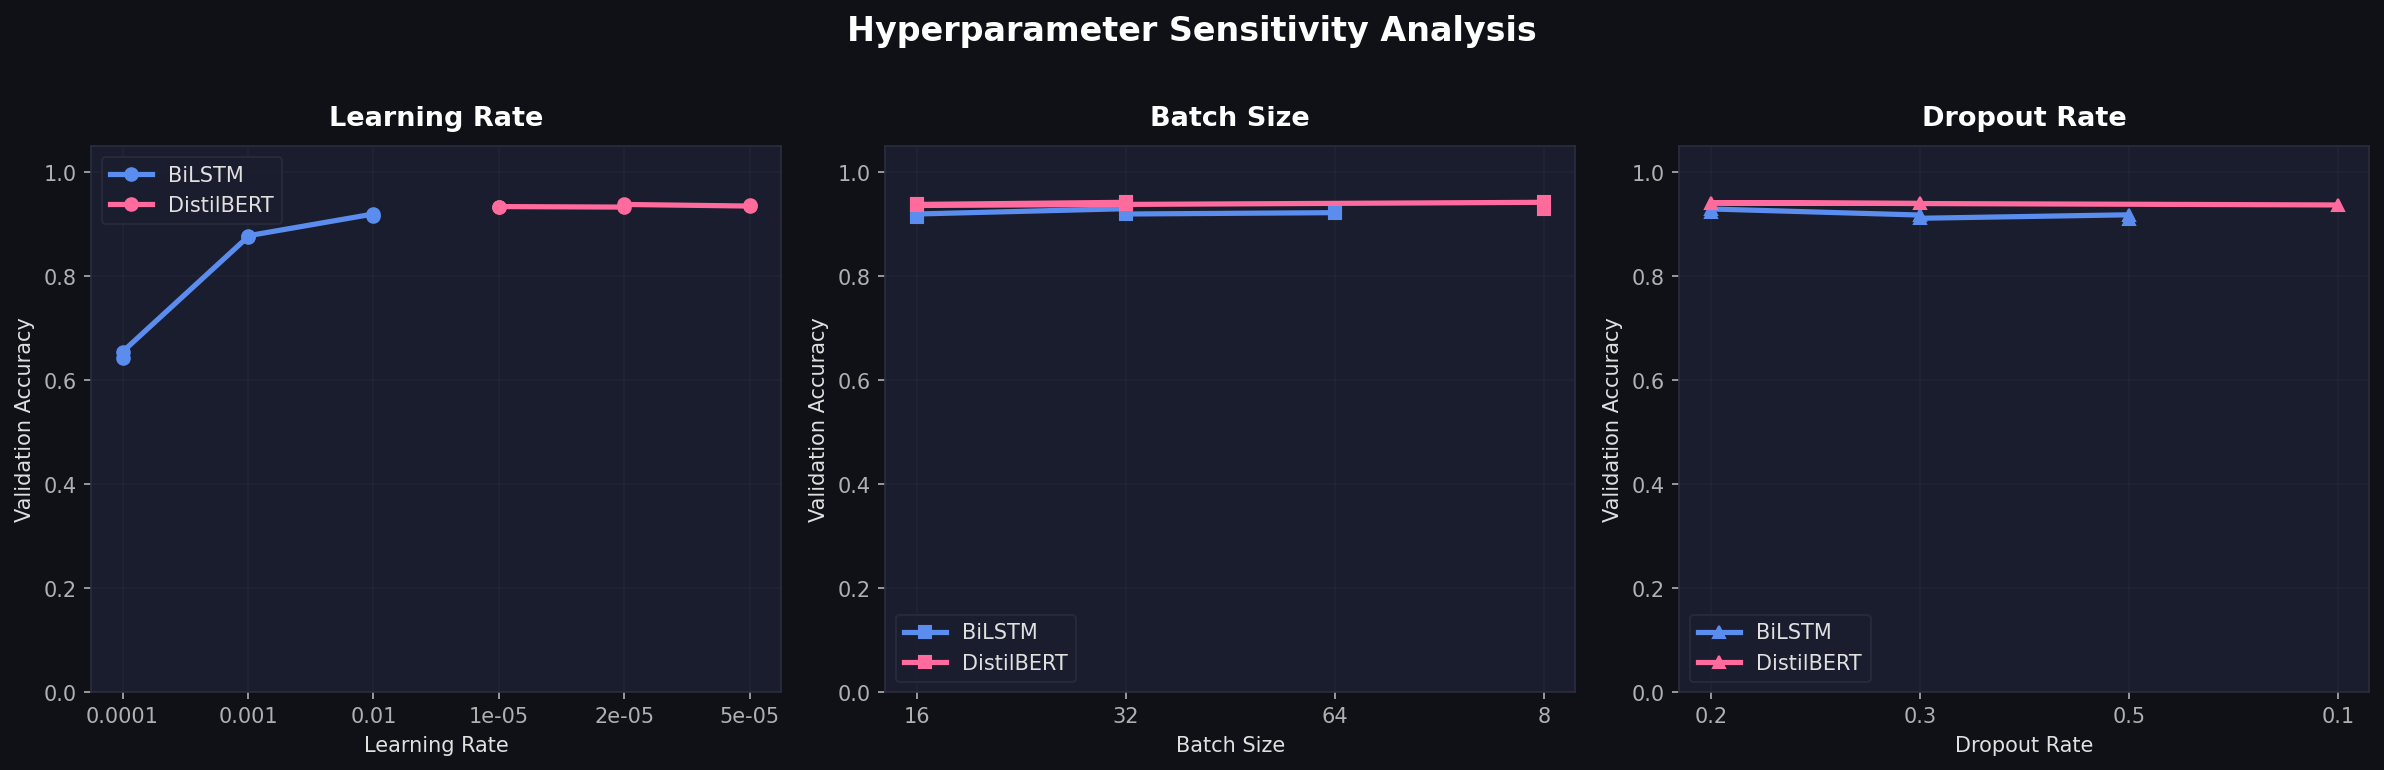
\includegraphics[width=0.9\textwidth]{../../figures/hyperparameter_sensitivity.png}
\caption{Hyperparameter Sensitivity Analysis}
\label{fig:hyperparam_sensitivity}
\end{figure}

%============================================
% REFERENCES
%============================================
\bibliographystyle{plain}
\begin{thebibliography}{9}

\bibitem{emotion_dataset}
Saravia, E., Liu, H.-C. T., Huang, Y.-H., Wu, J., \& Chen, Y.-S. (2018).
\textit{CARER: Contextualized Affect Representations for Emotion Recognition}.
In Proceedings of the 2018 Conference on Empirical Methods in Natural Language Processing.
\url{https://huggingface.co/datasets/dair-ai/emotion}

\bibitem{lstm}
Hochreiter, S., \& Schmidhuber, J. (1997).
\textit{Long Short-Term Memory}.
Neural Computation, 9(8), 1735-1780.

\bibitem{bilstm}
Schuster, M., \& Paliwal, K. K. (1997).
\textit{Bidirectional Recurrent Neural Networks}.
IEEE Transactions on Signal Processing, 45(11), 2673-2681.

\bibitem{distilbert}
Sanh, V., Debut, L., Chaumond, J., \& Wolf, T. (2019).
\textit{DistilBERT, a distilled version of BERT: smaller, faster, cheaper and lighter}.
arXiv preprint arXiv:1910.01108.

\bibitem{bert}
Devlin, J., Chang, M. W., Lee, K., \& Toutanova, K. (2018).
\textit{BERT: Pre-training of Deep Bidirectional Transformers for Language Understanding}.
arXiv preprint arXiv:1810.04805.

\bibitem{adam}
Kingma, D. P., \& Ba, J. (2014).
\textit{Adam: A Method for Stochastic Optimization}.
arXiv preprint arXiv:1412.6980.

\end{thebibliography}

\end{document}
